\documentclass{article}
\usepackage{graphicx} % Required for inserting images
\usepackage{wrapfig}
\usepackage{float}
\usepackage{pdflscape}
\usepackage[export]{adjustbox}
\usepackage{geometry}
\geometry{a4paper,
 total={170mm,257mm},
 left=5mm,
 top=20mm}
 \setcounter{secnumdepth}{5}
\usepackage{hyperref}
\title{Gruppo A (Micaela, Matteo, Paola, Marica)}
\author{Giovanni Cisternini}

\hypersetup{
    bookmarksopen = true
}

\begin{document}
\tableofcontents

\maketitle


\section{Nemici}
\begin{table}[h]
    \centering
    \begin{tabular}{cr|cr|cr|cr}
         \hypertarget{goblin}{Goblin}& \hypertarget{lupo}{Lupo} &\hypertarget{sildar}{Sildar}&\hypertarget{bugbear}{BugBear}\\
         \hline
           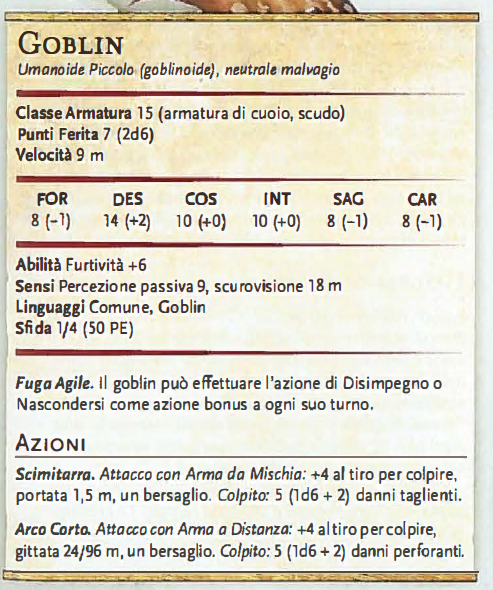
\includegraphics[width=4cm,height=6cm]{../Mostri/Goblin.png}  & 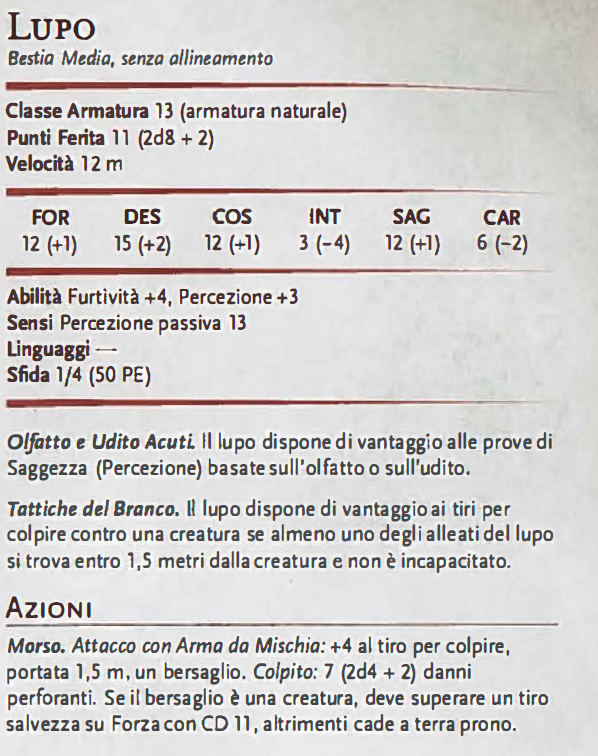
\includegraphics[width=4cm,height=6cm]{../Mostri/Lupo.png} & 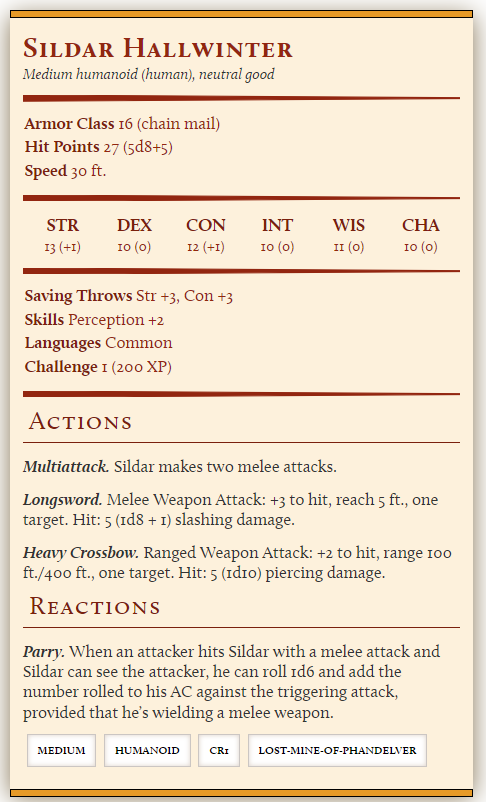
\includegraphics[width=4cm,height=6cm]{../PNG/Sildar_Hallwinter.png}&
            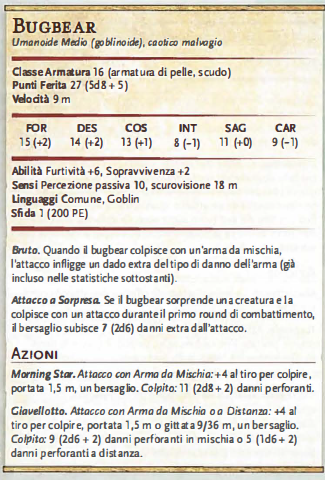
\includegraphics[width=4cm,height = 6cm]{../Mostri/Bugbear.png}\\
              \hline
            \hypertarget{marchirossi}{Marchi Rossi} & \hypertarget{orco}{Orco} & \hypertarget{ogre}{Ogre}&\hypertarget{kost}{Kost}\\
            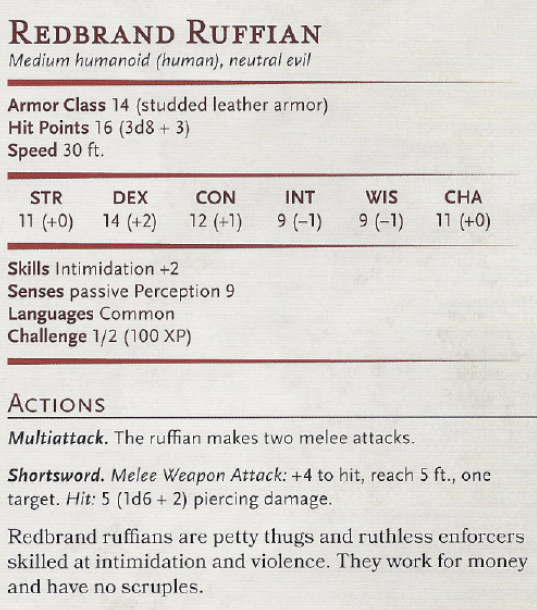
\includegraphics[width=4cm,height = 6cm]{../Mostri/Marchi Rossi.PNG} &  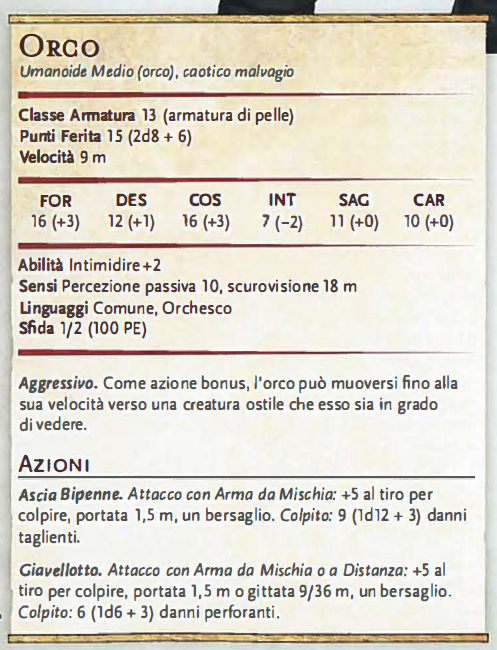
\includegraphics[width=4cm,height = 6cm]{../Mostri/Orco.PNG}& 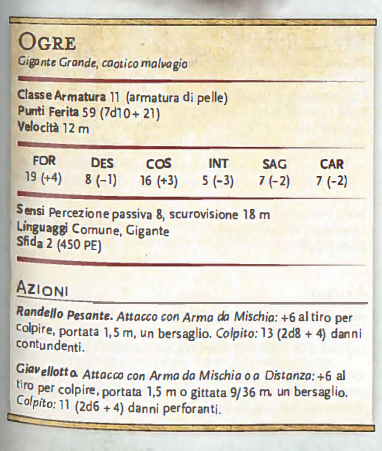
\includegraphics[width=4cm,height = 6cm]{../Mostri/Ogre.png}& 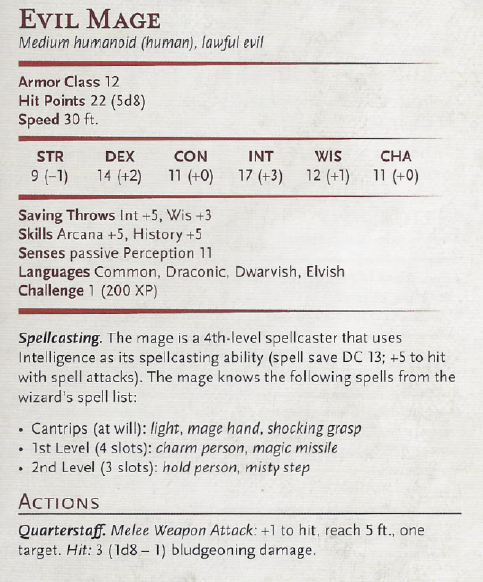
\includegraphics[width=4cm,height = 6cm]{../Mostri/HalmunKost.png} \\
              \hline
          
    \end{tabular}
     
\end{table}

\begin{table}
    \centering
      \begin{tabular}{cr|cr|cr|cr}
            \hypertarget{zombi}{Zombi} & \hypertarget{uccello}{Uccello Stigeo}&  \hypertarget{nothic}{Nothic} & \hypertarget{scheletro}{Scheletro}\\
            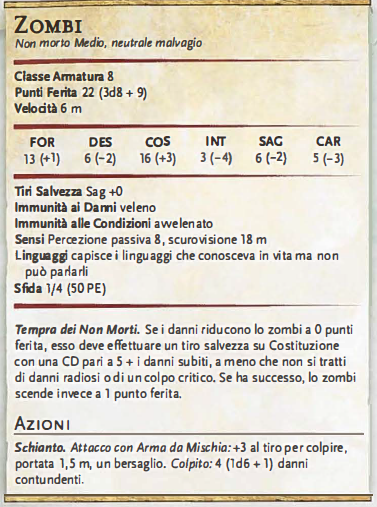
\includegraphics[width=4cm,height = 6cm]{../Mostri/Zombi.png}& 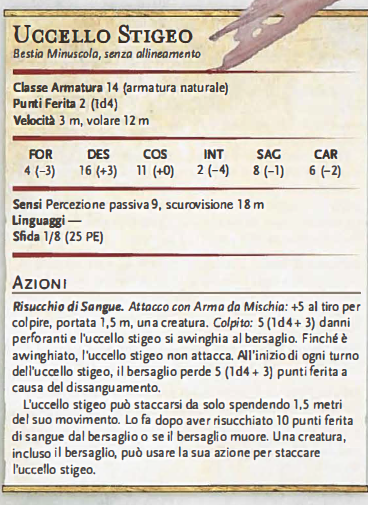
\includegraphics[width=4cm,height = 6cm]{../Mostri/UccelloStigeo.png}& 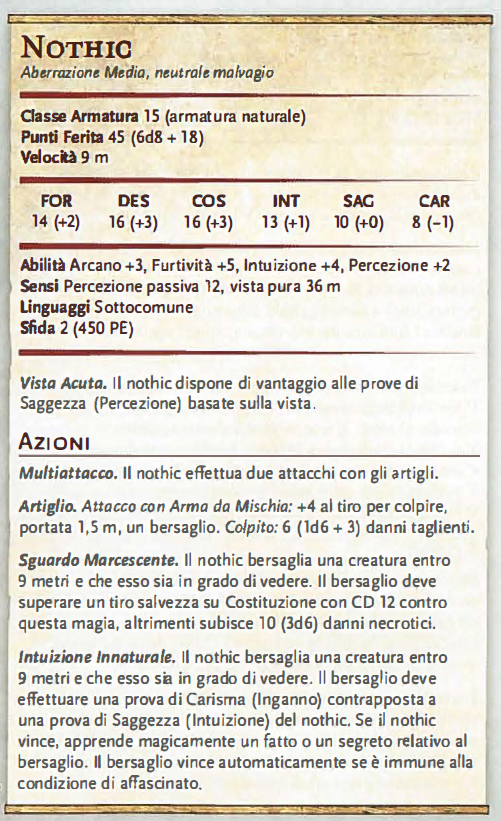
\includegraphics[width=4cm,height = 6cm]{../Mostri/Nothic.png}&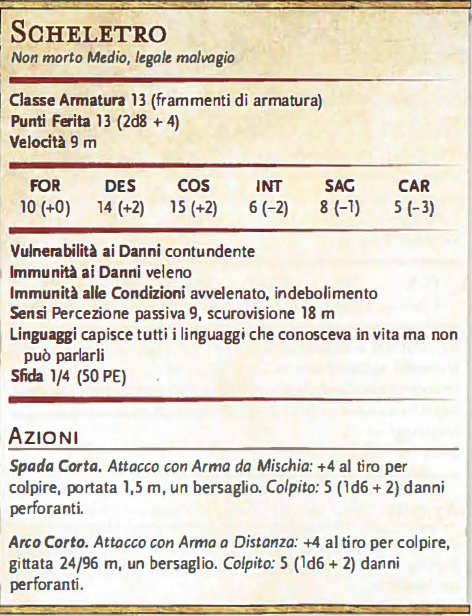
\includegraphics[width=4cm,height = 6cm]{../Mostri/Scheletro.png}\\
            \hline
              \hypertarget{Iarno}{Iarno} & \\
              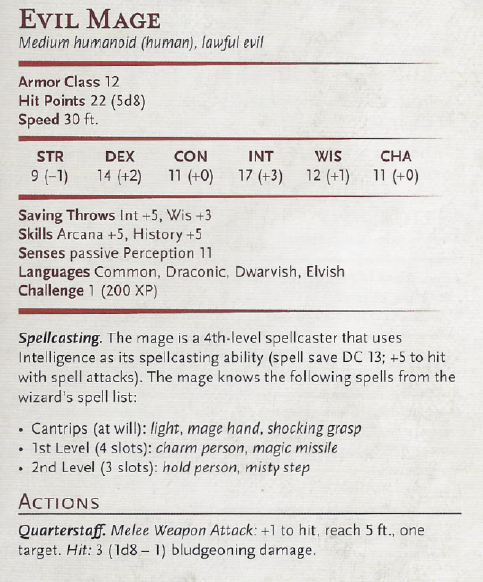
\includegraphics[width=4cm,height = 6cm]{../Mostri/HalmunKost.png}&\\
            
            
    \end{tabular}
\end{table}
\newpage
\section{PNG\_Compagni}
\subsection{Kai Serenestep}\hypertarget{kai}{Kai} è un monaco mezzelfo, orfano e addestrato fin da piccolo come monaco. I genitori sono completamente sconosciuti poiché era stato trovato in una cesta all'interno. I monaci che l'avevano trovato erano semplici eremiti non votati a nessuna vera religione, ma praticavano semplicemente la meditazione come forma di rilassamento e pace interiore per il ritrovamento dello spirito, aggiunta a produzione di vino e birra alquanto forti. L'aver vissuto con i monaci, gli ha insegnato a prendere la vita con allegria e spensieratezza, e soprattutto con molto vino. Una cosa turba profondamente Kai, i bulli, li odia fin da quando era bambino e veniva emarginato da alcuni bambini nel villaggio infondo alla valle. Si è comunque addestrato con i monaci fino all'età di 29-30 anni, finché non ha deciso di viaggiare per esplorare il mondo, l'unica cosa che sa è dove trovare alcool ma per il resto non ha la minima idea di come funzioni il mondo. Fisicamente è sul 1.80, con un fisico abbastanza scolpito, carnagione olivastra, con pantaloni invernali marroncini, delle bende alle mani, capelli rossastri, una bandana attorcigliata su se stessa legata intorno alla fronte, e un gilet di pelle con sotto una maglia abbastanza larga dello stesso corole dei pantaloni.  
\section{La miniera perduta di Phandelver (liv 1 - 5)}
\subsection{Inizio}
Il giorno dopo l'entrata a far parte degli avendwarfs: Cassiopea, Thia, Atalanta e Bryseis partono sotto comando di Thorgrim, per accompagnare il carro destinato a Phandalin, e per indagare sul messaggio ricevuto, portato dal gabbiano Ciro. Affrontano un primo viaggio di 2 giorni lungo la Strada Alta fino allo svincolo per la Pista di Triboar, si imbattono in 2 cavalli pieni di frecce e non si accorgono dell'imboscata dei goblin (combat).

Dopo il combattimento: 
    \begin{enumerate}
        \item Persuadono uno o più goblin oppure effettuano tiro \textsc{Sopravvivenza} CD 10 vanno al \hyperlink{cragmaw}{Il nascondiglio dei Cragmaw}
        \item Vanno direttamente verso \hyperlink{phandlin}{Phandalin}
        \item Hanno perso tutto vanno verso \hyperlink{phandalin}{Phandalin}
    \end{enumerate}

    \hypertarget{cragmaw}{\subsection{Il nascondiglio dei Cragmaw}}
    \begin{itemize}
        \item Meno di venti goblin vivono attualmente nella tana. CD 10
        \item  Il loro capo è un bugbear di nome Klarg, che risponde a Re
Grol, il capotribù dei Cragmaw, insediato nel Castello Cragmaw.
(I goblin possono fornire indicazioni generiche su come
raggiungere il Castello. Si trova a circa trenta chilometri a nordest
del nascondiglio dei Cragmaw, nel Bosco di Neverwinter.) CD 13
        \item Klarg ha ricevuto un messaggero goblin da Re Grol alcuni giorni fa. Il messaggero gli ha riferito che qualcuno che risponde al
nome di Ragno Nero aveva pagato i Cragmaw per intercettare il
nano Gundren Rockseeker, catturarlo e consegnare tutto ciò che portava con sé a Re Grol. Klarg ha obbedito agli ordini: ha teso
un'imboscata a Gundren e lo ha consegnato al re assieme ai suoi effetti personali, che includevano una mappa. CD 17
    \item Il nano e la sua mappa sono stati consegnati a Re Grol, come
da istruzioni. Il compagno umano del nano è tenuto prigioniero
nella “caverna dove si mangia” (l'area 6). 
    
    \end{itemize}
    \textbf{Tratti della caverna}
        \begin{enumerate}
            \item \textbf{Soffitti} Quasi tutte le caverne e i passaggi interni hanno soffitti inclinati che creato volto ricoperte di stalattiti, altezza tra i 6 e i 9 metri
            \item \textbf{Luce} Area 1 e 2 esterne. Il resto è immerso nell'oscurità, vedono se hanno scurovisione o una fonte di luce
            \item \textbf{Detriti} area di rocca franata e  ghiaia considerate terreno difficile
            \item \textbf{Suoni} Il fiume copre i rumori, per sentire \textsc{Percezione} CD 15
            \item \textbf{Stalagmiti} Colonne che possono fare da copertura
            \item \textbf{Torrente} Profondità di 60 cm, si guada facilmente
        \end{enumerate}
    \newpage
    \subsubsectionautorefname{Ingresso della caverna}
    \begin{figure}[t]
        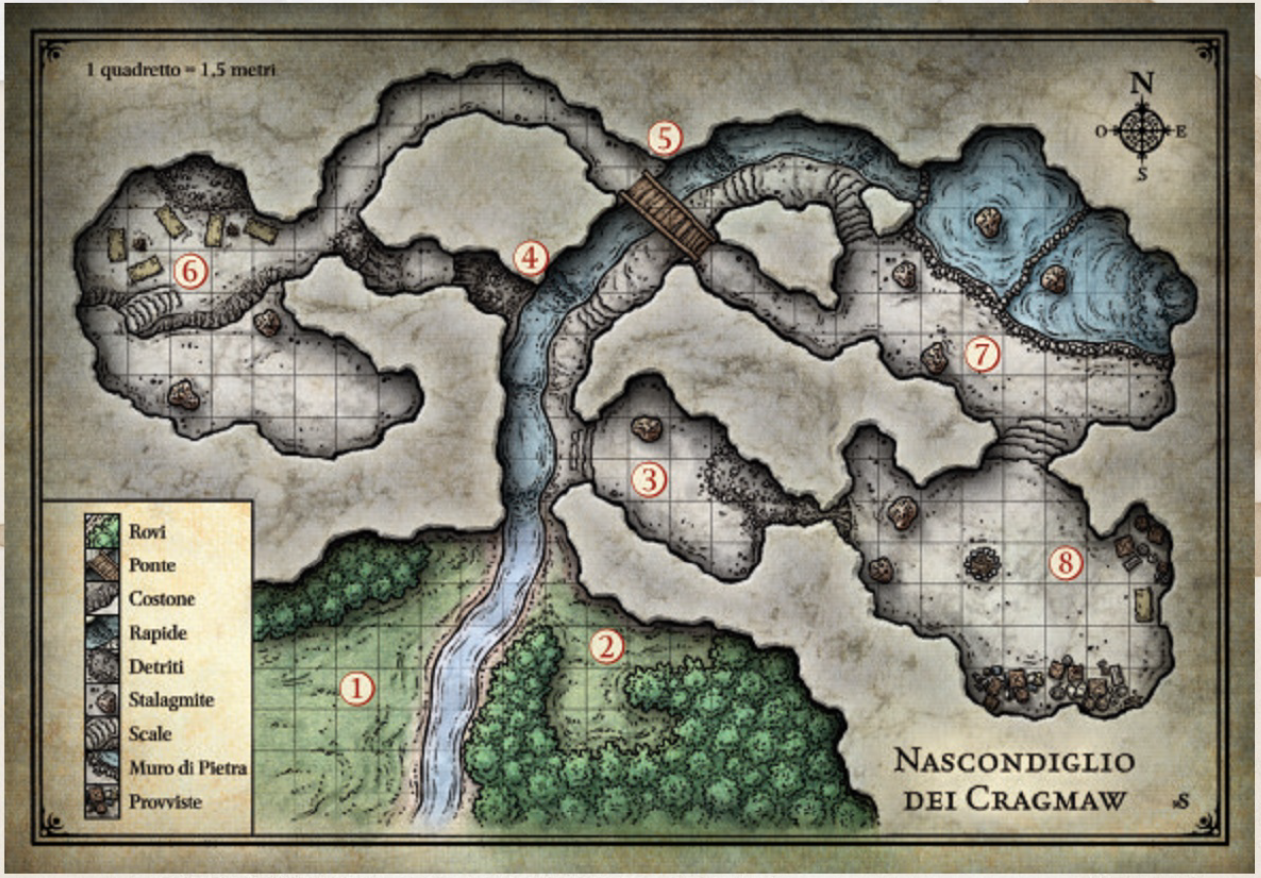
\includegraphics[width=20cm,height=12cm]{../Mappe/NascondiglioDiCagramaw.PNG}
    \end{figure}
        \textsc{Seguendo la pista dei goblin arrivate a una grande caverna che
si apre sul fianco della collina a circa sette chilometri e mezzo
dal punto dell’imboscata. Dall’ingresso della caverna scorre
un torrente quasi del tutto nascosto da folti cespugli di rovi.
Un esile sentiero asciutto che corre lungo la riva destra del
torrente conduce all’interno della caverna.}
\newline
\textbf{Sviluppi}
\newline
Nell'area 2 ci sono goblin, se i pg fanno tanto rumore i goblin si accorgono di loro e iniziano ad attaccare attraverso il roveto che fornisce mezza copertura +2 CA 
\subsubsection{Postazione Vedetta}
Se non vengono beccati dai goblin e passano al lato opposto, riescono a vedere i la vedetta oltre la cortina. Se i pg non camminano con prudenza allora i goblin li notano nell'area 2 e attaccano con gli archi. Prova di \textsc{Furtività} \newline \textsc{Sul lato est del torrente che scorre fuori dall’imboccatura della
caverna, una piccola area in mezzo al roveto è stata sgombrata
per formare una postazione di vedetta. Una serie di assi di
legno è stata stesa per appiattire i rovi e aprire uno spazio
sufficiente a consentire ai goblin di guardia di nascondersi
all’interno del roveto e di controllare l’area. Una coppia di
goblin occupa la postazione proprio ora!}



\subsubsection{Canile}
i cragmaw possiedono\textbf{4 lupi} \newline
\textsc{Subito dopo l’imboccatura della caverna, alcuni scalini di
pietra irregolari salgono fino a una fetida, piccola camera sul
lato est del passaggio. La caverna si restringe fino a diventare
una stretta crepa all’estremità più lontana ed è satura del
fetore di alcuni animali che devono vivere al suo interno. Alle
vostre orecchie giungonoi ringhi e lo sferragliare di catene di
tre lupi incatenati appena oltre l'apertura. La catena di ogni
lupo è legata a una verga di ferro piantata alla base di una
stalagmite.}\newline

- 3 lupi sono nell'area 3, non possono arrivare agli scalini perché sono legati, ma attaccano se un pg entra nell'area, se i pg provocano i lupi e tentano di attirarli fuori dall'area 3, i lupi provano a strappare la verga con prova su Forza (CD 15) finché vedono almeno un PG. Al primo successo la CD scende a 10. Al secondo il lupo si Libera. \newline
Se invece un PG tenta di calmare i lupi deve fare un tiro su \textsc{Addestrare animli} CD 15, se offrono del cibo la CD scende a 10, se superano i lupi lasciano passare i PG.\newline
\textbf{Crepa} C'è una crema in alto sul muro ad est, difronte agli scalini, che è sale di 9 metri fino all'area 8. Se provano a salire usando i detriti tiro su \textsc{Atletica} con CD 10, se la prova ha successo il personaggio può salire e scendere lungo il condotto, con risultato tra 6 e 9 resta immobile, con 5 o meno cade e si fa 1d6 di danno per ogni 3 metri di caduta, atterrando prono alla base del condotto.

\subsubsection{Passaggio Scosceso}
Da questo punto in avanti, i personaggi privi di scurovisione
avranno bisogno di luce per vedere cid che li circonda. \textsc{Il passaggio principale proveniente dall’imboccatura della
caverna sale ripidamente, mentre il ruscello si tuffa verso il
basso sul lato ovest, sollevando una pioggia di spruzzi. Tra
le ombre, un passaggio laterale conduce a ovest oltre la riva
opposta del ruscello.}\newline
I personaggi che usano la luce o la scurovisione per scrutare
lungo il passaggio notano il ponte nell’area 5. Il DM aggiunge
quanto segue: \textsc{Tra le ombre del soffitto a nord, riuscite a scorgere a malapena
la sagoma scura di un pericolante ponte di legnoe di corde
che attraversa il passaggio davanti a voi. Un altro passaggio si
incrocia con questo, a sei metri d’altezza dal terreno.}
Ogni personaggio che vede il ponte nell'area 5, fa un tiro su \textsc{Percezione} contrapposta alla prova \textbf{Furtività} dei goblin.
Il goblin nota i personaggi se hanno una fonte di luce o
non usano furtività quando si avvicinano al ponte. Il goblin
non attacca: tenta anzi di allontanarsi di soppiatto a est
per ordinare ai suoi compagni nell’area 7 di scatenare
un’\hyperlink{inondazione}{inondazione}.Il goblin si muove senza essere notato se la sua prova di
Destrezza (Furtività) è superiore al punteggio di Saggezza
(Percezione) passiva di qualsiasi personaggio che potrebbe
notare i suoi movimenti.\newline
\textbf{Passaggio Occidentale} Questo passaggio è occluso dai
detriti e da due costoni rocciosi molto ripidi. Quest'area
è considerata terreno difficile (vedi “Terreno Difficile” nel
regolamento).
La cornice tra i due costoni è fragile. Un qualsiasi peso
superiore a 50 chilogrammi fa cedere l’intera massa, che
cade rovinosamente verso est. Ogni creatura situata sulla
cornice quando questa crolla deve superare un tiro salvezza
su Destrezza con CD 10, subendo 2d6 danni contundenti in
caso di fallimento o soltanto la metà di quei danni in caso di
successo. Inoltre, in caso di tiro salvezza fallito, la creatura
cade a terra prona.

\subsubsection{Passaggio Rialzato}
IL ponte nell'area 5 è a 6 metri e incrocia il tunnel principale: \textsc{Il passaggio del torrente prosegue oltre un'altra serie di scalini
irregolari più avanti, curvando verso est. Da una caverna più
grande davanti a voi giunge il rumore rimbombante di una
cascata.}
Se non si erano accorti del ponte nell'area 4 se ne accorgono ora : \textsc{Un ponte malridotto si estende attraverso il passaggio,
collegando i due tunnel rialzati di 6 metri rispetto al torrente.} C'è un goblin di guardia che è nascosto. Furtivita Goblin VS Percezione PG. Se nessuno ha luci accessi e vanno in furtività allora il goblin non si accorge di nulla. \newline
\textbf{Ponte}. Collega 2 passaggi, situato a 6 metri, lo si può raggiungere scalando la parete rocciosa di metri, \textsc{Atletica }CD 15. il Ponte ha CA 5 e 10 PF se scende a 0 crolla e le creature tirano un TS su destrezza CD 10, se fallito 2d6 di danno, se superato si agrappa al ponte e si deve arrampicare CD 10

\hypertarget{inondazione}{\textbf{Inondazione}}\newline
    Le grosse vasche dell’area 7 sono dotate di pareti provvisorie
che possono essere abbattute tramite un meccanismo per
riversare un'ondata d’acqua nel passaggio principale della
tana. Nel round successivo a quello in cui ricevono il segnale
dalla vedetta nell’area 5, i goblin dell’area 7 iniziano a colpire
i pali di sostegno. Nel round successivo, al conteggio di
iniziativa dei goblin, un'ondata d’acqua si riversa dall'area 7
fino all'area 1.\newline
\textsc{Nel passaggio echeggia improvvisamente un possente boato e
una gigantesca ondata d’acqua si riversa su di voi dall’alto.}\newline
Linondazione minaccia tutte le creature nel tunnel (le
creature sul ponte dell’area 5 sono fuori pericolo, come
anche quei personaggi che riescono a scalare le pareti della
caverna). Ogni creatura entro 3 metri dal passaggio in disuso
nell’area 4 o dagli scalini che salgono fino all’area 3 può
effettuare un tiro salvezza su Destrezza con CD 10 per evitare
di essere spazzata via. Se una creatura non riesce a togliersi
di mezzo, può effettuare un tiro salvezza su Forza con CD 15
per tentare di aggrapparsi a qualcosa. In caso di fallimento, il
personaggio è buttato a terra prono e sospinto dall'acqua fino
all'area 1, subendo 1d6 danni contundenti lungo il cammino.
I goblin dell’area 7 possono scatenare una seconda
inondazione aprendo la seconda vasca, ma non lo fanno
a meno che non sia il goblin sul ponte a ordinarglielo. Il
goblin sul ponte aspetta di vedere se la prima inondazione
toglie di mezzo tutti gli intrusi prima di dare l'ordine di
aprire la seconda.
\subsubsection{Covo dei Goblin}
Dormitorio dei goblin : \textsc{Questa grande caverna è divisa in due da un costone alto tre
metri. Una ripida scalinata di pietra naturale sale dalla parte
più bassa alla cornice superiore. L'aria è densa del fumo di un
fuoco da campo e della puzza di pelli conciate rozzamente e di
goblin sporchi.}
\begin{itemize}
    \item 6 Goblin abitano questo covo, di cui , 5 nella parte più a nord che sono comuni, e 1, il capo, con 12 pf nella parte rialzata
    \item CAPO: Yeemik, tiene in ostaggio \textbf{Sildar Hallwinter} che 1 pf poiché è stato picchiato da dai goblin
\end{itemize}

Yeemik è il secondo in comando del nascondiglio, se capisce che sta per perdere la battagli, afferra Sildar e lo trascina al bordo della cornice superiore, grida : \textsc{Tregua, o questo
umano muore!”}.
Yeemik vuole spodestare Klarg e diventare il nuovo capo.
Se gli avventurieri accettano di trattare, Yeemik cerca
di convincerli a uccidere Klarg nell’area 8, promettendo
di liberare Sildar quando la testa del bugbear gli sarà
consegnata. Sildar, anche se stordito, avverte i personaggi
di non fidarsi del goblin, e ha buon motivo.Se i personaggi
stringono l'accordo, Yeemik cercherà di obbligarli a pagare un cospicuo riscatto per liberare Sildar, anche dopo che hanno
portato a termine quanto previsto dal patto.
Se i personaggi si rifiutano di trattare, Yeemik spinge
Sildar giù dal costone e continua a combattere. Sildar subisce
1d6 danni contundenti dalla caduta, sufficienti a portarlo
a 0 punti ferita. Se uno dei personaggi interviene in fretta,
può tentare di stabilizzarlo prima che muoia. \newline


\textbf{\title{Sildar Hallwinter}}
Sildar Hallwinter è un maschio umano di quasi
cinquant'anni, un uomo di buon cuore che occupa un posto
d'onore nella famosa cavalleria dei grifoni della grande città
di Waterdeep. È un agente dell'Alleanza dei Lord, un gruppo
di potenze politiche alleate al fine di garantire la prosperità e
la sicurezza reciproca. I membri dell'ordine garantiscono la
sicurezza delle città e degli altri insediamenti eliminando le
potenziali minacce in ogni modo e portando onore e gloria ai
loro capi e ai territori di provenienza.
Sildar ha incontrato Gundren Rockseeker a Neverwinter
e ha acconsentito di riaccompagnarlo a Phandalin. Sildar
desidera indagare sulla sorte di larno Albrek, un mago
umano che faceva parte dell'Alleanza dei Lord e che è
scomparso poco dopo essere arrivato a Phandalin. Sildar
spera di scoprire cos'è accaduto a larno, di aiutare Gundren
a riaprire la vecchia miniera e di incoraggiare Phandalin a
tornare ad essere un centro civilizzato e prosperoso.
Sildar fornisce ai personaggi quattro informazioni utili:
\begin{itemize}
    \item I tre fratelli Rockseeker (Gundren, Tharden e Nundro) di
recente avevano localizzato l'ingresso alla perduta Caverna
dell’Onda Tonante, che ospitava le miniere del Patto di
Phandelver.Più di cinquecento anni fa, i clan dei nani e degli gnomi
stipularono un accordo noto come il Patto di Phandelver, che
prevedeva la condivisione di una ricca miniera all’interno di
una meravigliosa caverna nota come la Caverna dell’Onda
Tonante. Oltre alle sue ricchezze minerarie, la miniera
conteneva grandi poteri magici. Alcuni incantatori umani si
allearono con i nani e gli gnomi per incanalare e vincolare
quell’energia a una grande forgia (chiamata la Forgia degli
Incantesimi), in grado di forgiare oggetti magici. Quelli
erano tempi prosperosi e anche il vicino paese di Phandalin
prosperava. Ma tutto finì nel disastro quando gli orchi
sciamarono in tutto il Nord e rasero al suolo tutto ciò che
incontrarono sul loro cammino.
Una potente banda di orchi che poteva contare sul supporto
di un gruppo di maghi mercenari malvagi attaccò la Caverna
dell’Onda Tonante per impossessarsi delle sue ricchezze e dei
suoi tesori magici. I maghi umani combatterono a fianco dei
nani e degli gnomi loro alleati per difendere la Forgia degli
Incantesimi, e la battaglia magica che ne seguì distrusse
buona parte della caverna. Pochi sopravvissero ai crolli e
alle scosse telluriche, e l'ubicazione della Caverna dell’Onda
Tonante andò perduta.
    \item Klarg, il bugbear che guida questa banda di goblin, aveva
l'ordine di tendere un'imboscata a Gundren. Sildar ha
sentito dire dai goblin cheIl Divoratore di Luce aveva dato l'ordine
che il nano gli fosse consegnato. Sildar non sa chi o cosa
siaIl Divoratore di Luce.
    \item Gundren possedeva una mappa che mostrava l'ubicazione
segreta della Caverna dell’Onda Tonante, ma i goblin
l'hanno portata via quando l’hanno catturato. Sildar crede
che Klarg abbia inviato la mappa e il nano al capotribù dei
Cragmaw in un luogo chiamato il Castello Cragmaw. Sildar
non sa dove possa trovarsi, ma presume che qualcuno a
Phandalin possa saperlo. (A Sildar non viene in mente
immediatamente, ma anche un goblin catturato potrebbe
essere persuaso a rivelare l'ubicazione del castello. Vedi il
riquadro “Cosa Sanno i Goblin” a pagina 8.)
\item Il contatto di Sildar a Phandalin è un mago umano di nome
larno Albrek. Il mago si era recato in paese due mesi fa
per fare ordine nel posto. Quando l'Alleanza dei Lord non
ha ricevuto più alcuna notizia da larno, Sildar ha deciso di
indagare.
\end{itemize}
\newpage
\textbf{\title{Alleanza dei Lord}}
L'Alleanza dei Lord non è una nazione in sé, beni una rete dei governaotori di vari paesi e città che hanno giurato di mantenere la pace gli uni con gli altri e di condividere informazioni e risorse contro minacce comuni, come le orde degli orchi e i pirati Nordici. È una conferederazione semiufficiosa di quegli insediamenti e dei loro agenti che giurano tutti fedeltà ai loro territori natii per primi e all'Alleanza dei Lord per seconda.


\textbf{\title{Sviluppi}}
Sildar salvato si unisce al gruppo, e chiede di essere scortato a Phandalin il prima possibile. Non ha armi ma può prendere le armi dei goblin o prendere in prestito un arma di un personaggio

\textbf{\title{Tesoro}}Yeemik porta con sé un borsello contenente tre denti d’oro
(1 mo ciascuno) e 15 ma. L'equipaggiamento di Sildar è stato
portato al Castello Cragmaw assieme a Gundren Rockseeker.

\subsubsection{Caverna delle Due Vasche}
Se le vasche sono `già svuotate devo modificare il disegno con un riquadro nero sopra e modificare il testo : \textsc{Questa caverna è occupata per metà da due grandi vasche
piene d’acqua. Una piccola cascata sulla parte alta della parete
est alimenta le vasche, che si svuotano all’estremità opposta
per formare il torrente che poi esce dall'imboccatura della
caverna, più in basso. Due bassi muretti di pietre fungono da
dighe che trattengono l’acqua. A sud si apre un’ampia uscita
mentre due passaggi più piccoli conducono a ovest. Il rumore
della cascata echeggia per tutta la caverna e rende più difficile
udire gli altri rumori.}

In questa caverna ci sono 3 goblin, se sono stati avverti precedentemente dal goblin dell'area 5 allora sono già pronti a combattere, altrimenti sono distratti. La cascata copre il rumore dei combattimenti quindi nell'area 8 non si sente nulla, ma un goblin può scappare e tentare di avvisare Klarg.

\subsubsection{Caverna di Klarg}
Capo dei goblinoidi che conserva il grosso delle merci rubate nella sua caverna.
\textsc{Lungo la parete sud di questa vasta caverna sono stati
accumulati i sacchi e le casse di provviste rubate. A ovest, il
pavimento scende gradualmente verso una stretta apertura
che si inoltra nell'oscurità. Un’apertura più grande che conduce
verso una scalinata di pietra naturale si apre a nord. Da quel lato
proviene il rombo di una cascata. Al centro della caverna ardono
le braci di quello che un tempo doveva essere un grande falò.}\newline

\textbf{Klarg} bugbear, che condivide la sua caverna con un lupo Squartatore, e 2 goblin. Ha manie di grandezza e parla in terza persona.\newline
\textbf{Fossa falo}, se ci passi sopra 1 danno, ci cadi dentro 1d6, è al centro della stanza
\textbf{Condotto naturale} dell'area 3
\textbf{Provviste}Le casse e i sacchi
impilati gli uni sugli altri
possono fornire metà copertura
a qualsiasi creatura che
combatta o si nasconda dietro
di essi. Molti sono decorati
con l'immagine di un leone
azzurro, il simbolo dello Scudo
del Leone, una compagnia
mercantile che possiede un
magazzino e un avamposto
commerciale a Phandalin.
Tra le provviste è nascosto
un forziere del tesoro che
‘apparteneva a Klarg (vedi la
sezione “Tesoro”) e non è chiuso
a chiave. Qualsiasi personaggio
che esamini le provviste
trova il forziere.



\textbf{\title{Sviluppi}} 
Se Klarg è stato avvertito, lui e il lupo si nascondono tra le stalagmiti e i goblin fra le provviste, e provano a tendere un'imboscata 
Se non viene avvertito possono sorprenderli, il modo più facile è usando il condotto dell'area 3. Se il lupo viene ucciso il bugbear prova a scappare dal condotto.

\textbf{\title{Tesoro}}
Scorte, sono molte, hanno bisogno di un carro per trasportarle. 
Se restituiscono le scorte allo Scudo del LEone ottengono 50 mo e l'amicizia di Linene e della sua compagnia.
Klarg ha aanche forziere con 600 mr, 110 ma due pozioni di guarigione e una statuetta di giada che raffigura una rana con due minuscoli globi dorati al posto degli occhi ( 40 mo) , può andare in tasca
\newpage
\subsection{Phandalin}
        \begin{table}
            \centering
            \begin{tabular}{|c|c|c|}
            \hline 
            \multicolumn{3}{|c|}{Guest}\\
            \hline  
                 Sorella Gareale & Il Patto con le Banshee &  \\
            \hline
                 Daran Edermath & Problemi al Vecchi Gufo & X\\
            \hline
                 Harbin Wester & Problemi con Gli orchi & \\
            \hline
                 Halia Thornton & Offerta di Lavoro &\\
            \hline 
            
            \hline
            \end{tabular}
           
        \end{table}
        
       \begin{figure}[ht] 
        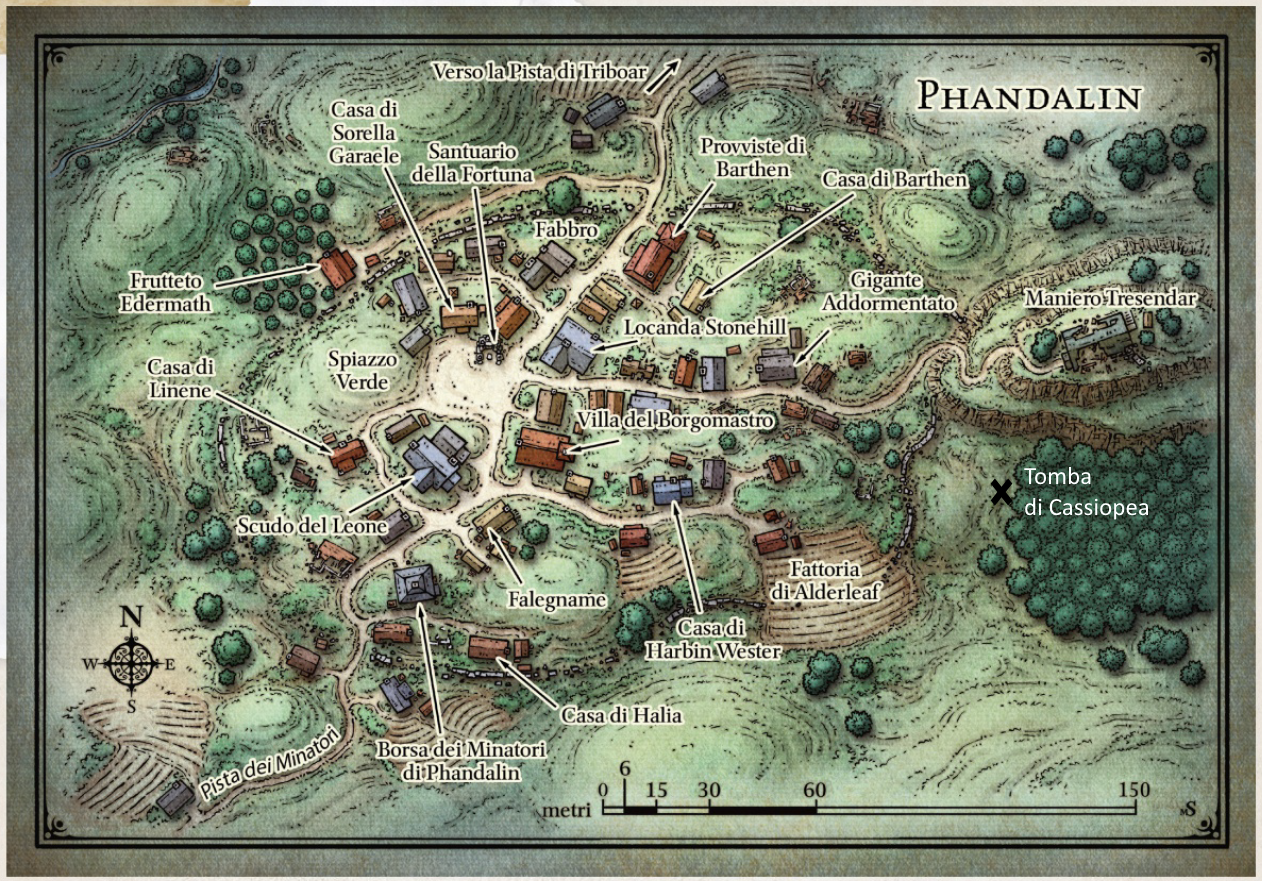
\includegraphics[scale=0.75, left]{../Mappe/Phandalin.PNG}
        \end{figure}

        \subsubsection{Descrizione Per Phandalin}
        \textsc{Il sentiero dissestato supera il fianco boscoso di una collina
        e vi rivela il paese di Phandalin, composto da quaranta o
        cinquanta semplici edifici di legno, alcuni dei quali eretti su
        vecchie fondamenta di pietra. Altre vecchie rovine (mura di
        pietra diroccate ricoperte di edera e rovi) circondano le case e
        le botteghe più nuove, a testimonianza del fatto che nei secoli
        passati il paese doveva essere molto più grande. La maggior
        parte dei nuovi edifici sorge lungo il sentiero, che si allarga
        fino a diventare una sorta di fangosa via principale e sale verso
        un maniero diroccato che sorge sul fianco di una collina sul
        lato orientale del paese.
        Quando vi avvicinate, vedete dei bambini che giocano in
        uno spiazzo verde in mezzo al paese e alcuni cittadini intenti
        a lavorare o a sbrigare commissioni presso qualche bottega.
        Molti alzano la testa al vostro arrivo, ma riprendono a lavorare
        al vostro passaggio.} 
I personaggi
arrivano a sera inoltrata e non potranno visitare più di uno o 
due luoghi prima di cercare alloggio per la notte.\newline
Alcuni luoghi che i personaggi possono visitare sono
i seguenti:
\begin{enumerate}
    \item \hyperlink{provviste}{Provviste di Barthen}. Se i personaggi sono in possesso del
carro di provviste dell’aggancio per l'avventura “Ci Vediamo
a Phandalin”, devono consegnarlo a questo negozio.
`\item Scudo del Leone. Se i personaggi hanno recuperato le
merci rubate dal nascondiglio dei Cragmaw, potrebbero
decidere di restituirle al legittimo proprietario.
\item Locanda Stonehill. Se i personaggi sono accompagnati
da Sildar Hallwinter, il cavaliere suggerisce loro di visitare
questa locanda per trovare una sistemazione. Se cercano
per altre vie un luogo dove mangiare e dormire, scoprono
che la Locanda Stonehill sembra essere la migliore opzione
disponibile.
\end{enumerate}
\subsubsection{PNG\_PHANDALIN}
\begin{table}[h]
    
    \begin{tabular}{|c|p{10cm}|}
        \hline
      X Toblen Stonehill &  Locandiere\\
       \hline
Elmar Barthen  & Proprietario di un avamposto commerciale;
deve dei soldi al gruppo, se è stato usato
l’aggancio per l'avventura “Ci Vediamo a
Phandalin”.   \\
    \hline
        Daran Edermath & Membro dell'Ordine del Guanto d’Arme. Ha
una missione per il gruppo .\\
    \hline
    Linene Graywind & Gestisce un avamposto commerciale e
offre una ricompensa a chi recupera le sue
provviste.\\
    \hline
    Halia Thornton & Membro degli Zhentarim. Ha una missione
per il gruppo.\\ \hline
X Qelline Alderleaf & Premurosa contadina halfling il cui figlio,
Carp, conosce un passaggio segreto che
conduce al nascondiglio dei Marchi Rossi.\\ \hline
Sorella Garaele & Elfa chierica di Tymora e agente degli Arpisti.
Ha una missione per il gruppo. \\ \hline
Harbin Wester & Borgomastro di Phandalin. Ha una missione
peril gruppo. \\ \hline
    \end{tabular}
\end{table}



\subsubsection{Fabbro: Il Martellatore}
\subsubsection{Falegname: La sega umana}

\subsubsection{Locanda Stonehill}
\subparagraph{Presentazione}
Al centro del paese si erge una grossa locanda costruita di
recente, fatta di pietra e di rozze travi di legno. La sala comune
è affollata di abitanti locali che sorseggiano un boccale di sidro
o di birra e vi osservano incuriositi.

\subparagraph{Descrizione}
Questa modesta locanda è dotata di sei camere disponibili
. Se i personaggi decidono
di pernottare qui, vedi la tabella “Vitto e Alloggio” nel
regolamento peri prezzi. (In alternativa i personaggi possono
accamparsi fuori dal paese o convincere un contadino come
Daran Edermath o Qelline Alderleafa lasciarli dormire
in un fienile)
Il locandiere è un giovane umano basso e cordiale di nome
Toblen Stonehill, che proviene dal paese di Triboar a est.
È giunto a Phandalin come cercatore minerario, ma presto
ha capito che era molto più abile nel gestire una locanda
che una miniera. Il nuovo paese gli ha offerto una buona
opportunità di sistemarsi. Toblen è irritato dal fatto chei
Marchi Rossi possano terrorizzare il paese indisturbati e
che Harbin Wester, il borgomastro, non abbia fatto niente per
contrastarli. Tuttavia, cerca di non attirare troppo l’attenzione
su di sé, nel timore che i Marchi Rossi possano scatenare una
rappresaglia contro sua moglie e i suoi figli

\subparagraph{Dicerie}
Passando un po’ di tempo nella sala comune a
chiacchierare con gli abitanti, i personaggi possono scoprire
varie tracce interessanti sui luoghi da esplorare in paese e nei
dintorni. I PNG presenti alla Locanda Stonehill e le dicerie
che possono rivelare includono quanto segue:
\begin{enumerate}
    \item Elsa, una cameriera chiacchierona: “Daran Edermath, il
custode del frutteto, è un vecchio avventuriero.” (Vedi la
sezione “\hyperlink{frutteto}{Frutteto Edermath}” per ulteriori informazioni.)[X]
    \item Narth, un vecchio contadino: “Sorella Garaele, che presiede
il Santuario della Fortuna, di recente ha lasciato il paese
per qualche giorno, poi ha fatto ritorno ferita e stremata.”
(Vedi la sezione “\hyperlink{santuario}{Santuario della Fortuna}” per ulteriori
informazioni.)[]
\item Pip, il giovane figlio di Toblen: “Il figlio di Qelline Alderleaf,
Carp, ha detto di avere trovato un tunnel segreto nei boschi,
ma i Marchi Rossi lo hanno quasi catturato.” (Vedi la
sezione “\hyperlink{fattoria}{Fattoria Alderleaf}” per ulteriori informazioni)[X]
\item Trilena, la moglie del locandiere: “Thel Dendrar, un
intagliatore di legno locale, ha tenuto testa ai Marchi Rossi
una decade fa, quando si sono presentati nel suo negozio e
hanno molestato sua moglie. E i malviventi allora l'hanno
ucciso. Alcuni abitanti hanno visto tutto. I Marchi Rossi
hanno portato via il cadavere, e ora anche sua moglie, suo
figlio e sua figlia sono scomparsi.” (All’insaputa di Trilena e
degli altri abitanti, i Marchi Rossi hanno portato la moglie e
i figli di Thel nel loro nascondiglio segreto.)[] Sera in cui rivedono Lirael
\item Freda, una tessitrice: “I Marchi Rossi molestano ogni
bottega in paese, ad eccezione della Borsa dei Minatori di
Phandalin. Non vogliono avere guai con Halia Thornton,
che la gestisce.” (Vedi la sezione “\hyperlink{borsa}{Borsa dei Minatori di
Phandalin}” per ulteriori informazioni).[] 
    \item Lanar, un minatore: “Alcuni orchi razziatori sono stati
avvistati all'estremità est della Pista di Triboar. Il
borgomastro cerca qualcuno che li metta in fuga.” (Vedi la
sezione "\hyperlink{villa}{Villa del Borgomastro}” per ulteriori informazioni.)[]
    


\end{enumerate}

\subsubsection{PROVVISTE DI BARTHEN}
\hypertarget{provviste}{}
Quello di Barthen è il più grande avamposto commerciale
di Phandalin. Sui suoi scaffali sono disponibili le merci e le
provviste più comuni, dagli zaini ai giacigli, dalle corde alle
razioni. Il negozio è aperto dall’alba al tramonto. Barthen non
vende armi o armature, ma i personaggi possono comprare
da lui tutto il resto dell’equipaggiamento d’avventura, ad
eccezione degli oggetti dal costo superiore a 25 mo. (Vedi
“Equipaggiamento d’Avventura” nel regolamento peri
relativi prezzi.) Quei personaggi che hanno bisogno di armi
o armature vengono indirizzati allo Scudo del Leone (vedi la
relativa sezione).
Il proprietario del negozio è \textbf{Elmar Barthen}, un umano
magro e calvo, dai modi gentili, sulla cinquantina. Tiene in
negozio un paio di giovani commessi (Ander e Thistle), che
lo aiutano a caricare e scaricare i carri e servono i clienti
quando il titolare non è in negozio.
\subparagraph{Consegnare le Provviste}
Se i personaggi hanno iniziato
a giocare con l'aggancio per l'avventura “Ci Vediamo a
Phandalin”, hanno l’ordine di consegnare il carro di provviste
al negozio di Barthen. Il venditore paga la cifra concordata
(10 mo a ogni personaggio) e prende possesso sia del carro
che delle provviste. Se i personaggi gli parlano della cattura
di Gundren Rockseeker, Barthen è rattristato dalla notizia
e incoraggia il gruppo a trovare e salvare il nano. Considera
Gundren un amico e aveva appreso con entusiasmo la notizia
della scoperta della miniera perduta del Patto di Phandelver
tra le colline circostanti. Se il gruppo non ha ancora appreso
i dettagli della miniera da Sildar Hallwinter, un personaggio
può superare una prova di Intelligenza (Storia) con CD 15
per riferire le informazioni: \textbf{Più di cinquecento anni fa, i clan dei nani e degli gnomi
stipularono un accordo noto come il Patto di Phandelver, che
prevedeva la condivisione di una ricca miniera all’interno di
una meravigliosa caverna nota come la Caverna dell’Onda
Tonante. Oltre alle sue ricchezze minerarie, la miniera
conteneva grandi poteri magici. Alcuni incantatori umani si
allearono con i nani e gli gnomi per incanalare e vincolare
quell’energia a una grande forgia (chiamata la Forgia degli
Incantesimi), in grado di forgiare oggetti magici. Quelli
erano tempi prosperosi e anche il vicino paese di Phandalin
prosperava. Ma tutto finì nel disastro quando gli orchi
sciamarono in tutto il Nord e rasero al suolo tutto ciò che
incontrarono sul loro cammino.
Una potente banda di orchi che poteva contare sul supporto
di un gruppo di maghi mercenari malvagi attaccò la Caverna
dell’Onda Tonante per impossessarsi delle sue ricchezze e dei
suoi tesori magici. I maghi umani combatterono a fianco dei
nani e degli gnomi loro alleati per difendere la Forgia degli
Incantesimi, e la battaglia magica che ne seguì distrusse
buona parte della caverna. Pochi sopravvissero ai crolli e
alle scosse telluriche, e l'ubicazione della Caverna dell’Onda
Tonante andò perduta.}
Barthen aggiunge inoltre che altri due fratelli Rockseeker,
Nundro e Tharden, si sono accampati da qualche parte fuori
città. Non li vede da una decade e si aspetta che tornino ormai
“da un giorno all’altro” per fare rifornimento. Ciò che Barthen
non sa è che Tharden è morto e Nundro è tenuto prigioniero
nella miniera. Vedi nella quarta parte, la sezione “La Caverna
dell’Onda Tonante” per ulteriori informazioni.
\subparagraph{Le Notizie di Barthen}
Se i personaggi chiedono a Barthen
come vanno gli affari, il negoziante risponde che i Marchi Rossi rendono la vita difficile a tutti, riscuotendo il pizzo dai
negozi locali e facendosi beffe dell'autorità del borgomastro. Se
i personaggi sembrano intenzionati a intervenire, aggiunge che
i Marchi Rossi frequentano l’osteria del Gigante Addormentato

\subsubsection{Frutteto Edermath}
\hypertarget{frutteto}{}
Daran Edermath è un avventuriero a riposo che vive in una
casetta ai margini di un frutteto di meli. Daran, un atletico
mezzelfo dai capelli d’argento più che centenario, è un
guerriero che ha prestato servizio come sceriffo e araldo per
molti anni nei territori della Costa del Drago, nel lontano
sudest. Quando ha deciso di ritirarsi, ha fatto ritorno alla
regione di Neverwinter, la sua terra d’origine.
Daran è un membro dell'Ordine del Guanto d’Arme,
un gruppo di instancabili sorveglianti che ha lo scopo di
proteggere il prossimo dalle aggressioni dei malfattori.
L'ordine vigila costantemente, pronto a punire il male, a
far rispettare la giustizia e a lanciare rappresaglie contro
chiunque tenti di sottomettere o fare del male agli altri. Anche
se non fa più attivamente parte dell'ordine, Daran cerca
comunque di tenere d'occhio gli eventi nella zona di Phandalin.
Condivide volentieri le notizie con gli altri avventurieri,
specialmente se sembrano aderire ai suoi stessi principi.
Daran è preoccupato per i Marchi Rossi e vorrebbe che
un gruppo di avventurieri insegnasse a quei malviventi una
lezione. Spiega ai personaggi che è ora che qualcuno affronti
Bastone di Vetro, il capo dei Marchi Rossi. Daran sa che i
Marchi Rossi frequentano l’osteria del Gigante Addormentato,
ma può rivelare ai personaggi anche che il rifugio principale
dei Marchi Rossi si trova sotto il Maniero Tresendar, un
complesso di rovine situato ai margini orientali del paese. (Vedi
la sezione “\hyperlink{maniero}{Maniero Tresendar}” per ulteriori informazioni.)
\subparagraph{Problemi al Vecchio Gufo}
 A Daran sono giunte
voci dai cercatori minerari attivi sulle colline a nordest di
Phandalin: qualcuno starebbe effettuando degli scavi tra le
rovine note come il Pozzo del Vecchio Gufo. Ma soprattutto,
cosa più inquietante, vari cercatori avrebbero riferito di
essere stati scacciati dall'area da alcune creature non morte.
Daran chiede ai personaggi di visitare le rovine, un viaggio
di due giorni di marcia a nordest di Phandalin, e di scoprire
cosa sta succedendo. Daran sa che le rovine appartengono
a una vecchia torre di guardia di un antico impero magico
noto come Netheril, e teme che possano racchiudere qualche
pericolosa magia latente. Se il gruppo intraprende questa
missione, vedi “\hyperlink{gufo}{Il Pozzo del Vecchio Gufo}”

\subparagraph{Conseguenze: UNIRSI ALL'ORDINE DEL GUANTO D'ARME }
Se il gruppo ha a che fare con i Marchi Rossi e indaga sul
Pozzo del Vecchio Gufo, Daran Edermath contatta alcuni
membri del gruppo e li invita a unirsi all'Ordine del Guanto
d’Arme. Parla con quelli che a sua detta rappresentano
meglio le virtù dell'ordine, come l'onore e la vigilanza. Se un
personaggio accetta, Daran gli conferisce il titolo di Chevall.  

\subsubsection{Scudo del Leone}
\subparagraph{Descrizione}
Sopra la porta d’ingresso di questo modesto avamposto
commerciale pende un'insegna a forma di scudo di legno su
cui è stato dipinto un leone azzurro.
\subparagraph{Missione}
Questo edificio è di proprietà dello Scudo del Leone, una
compagnia mercantile che ha sede nella città di Yartar, oltre
centocinquanta chilometri più a est. La compagnia spedisce
prodotti finiti a Phandalin e ad altri piccoli insediamenti in
tutta la regione, ma questo avamposto di recente è finito nelle
mire dei banditi. L'ultima carovana dello Scudo del Leone
che doveva arrivare a Phandalin non è mai arrivata. (È stata
attaccata e il suo carico è stato catturato dai goblin Cragmaw.)
La responsabile dell’avamposto di Phandalin è una donna
dalla lingua tagliente, di circa trentacinque anni, di nome
Linene Graywind. Sa che alcuni banditi hanno assalito
le carovane dello Scudo del Leone, ma non sa chi sia il
responsabile.
Linene custodisce in una stanza sul retro una piccola
scorta di armi e armature, disponibili peri compratori
interessati. (Vedi “Equipaggiamento d’Avventura” nel
regolamento peri prezzi.) Linene però ha qualche scrupolo e
non venderà le armi a chi considera una potenziale minaccia
per il villaggio. Di conseguenza si rifiuta di fare affari con
i Marchi Rossi. Mette in guardia i personaggi contro i
malviventi e consiglia loro di evitare l’osteria del Gigante
Addormentato.
\subparagraph{Merci Recuperate}. Se i personaggi restituiscono le merci
rubate trovate nell’area 8 del nascondiglio dei Cragmaw (o se
hanno lasciato le merci sul posto, ma spiegano a Linene dove
trovarle), ottengono dalla donna una ricompensa di 50 mo e
la promessa di aiutare gli avventurieri in ogni modo che le
sia possibile.
\subsubsection{Borsa dei minatori Di Phandalin}
\hypertarget{borsa}{}
La Borsa dei Minatori è un avamposto commerciale dove
i minatori locali possono far pesare, misurare e vendere i
metalli estratti. In assenza di un qualsiasi nobile o autorità
locale, la borsa funge anche da ufficio del catasto informale,
registrando le concessioni di vari ruscelli e siti di scavo
nell’area. Quella di Phandalin non può essere definita una
vera e propria febbre dell'oro, ma i corsi d’acqua e le valli vicine nascondono abbastanza ricchezze da mantenere un
buon numero di cercatori indipendenti.
La borsa é un ottimo posto dove incontrare gente che passa
molto tempo nelle campagne attorno a Phandalin. La maestra
di gilda è una donna ambiziosa e calcolatrice di nome Halia
Thornton. Nel tentativo di fare della Borsa dei Minatori la
cosa più vicina a un'autorità governativa che il paese possa
avere, si atteggia a ben più di una semplice mercante. È
inoltre un'agente degli Zhentarim, una potente organizzazione
segreta che cerca di ottenere il controllo sul Nord attraverso
la ricchezza e l'influenza economica. Halia vuole portare
gradualmente Phandalim sotto il suo controllo e può diventare
una preziosa datrice di lavoro per i personaggi, se questi si
dimostrano gente di parola con lei.
Halia non sa dove si trovi il Castello Cragmaw, ma ha
sentito dire che i Marchi Rossi tengono un goblin al loro
servizio. Forse il goblin in questione potrebbe sapere dove
si trova il castello. Halia cerca di fare buon uso di questa
informazione per persuadere i personaggi ad aiutarla a
occuparsi dei Marchi Rossi.
\subparagraph{Missione: L’Offerta di Lavoro di Halia.}Se contattata
da personaggi che crede di poter controllare, Halia spiega
che i Marchi Rossi sono un problema. Racconta di come i
malviventi si radunino all’osteria del Gigante Addormentato
e possiedano una base sotto il Maniero Tresendar, ai confini
orientali del paese. Poi offre ai personaggi 100 mo per
eliminare il capo dei Marchi Rossi, quello che i fuorilegge
chiamano Bastone di Vetro, e consegnarle gli eventuali
carteggi che troveranno negli alloggi del capobanda. Halia
non rivela che ha intenzione di mettersi personalmente
al comando dei Marchi Rossi. Una prova di Saggezza (Intuizione) con CD 15 consente a un personaggio di capire
che la donna potrebbe avere ulteriori motivi per togliere di
mezzo il capo dei Marchi Rossi.

\subparagraph{UNIRSI AGLI ZHENTARIM}
Se il gruppo si sbarazza del capo dei Marchi Rossi, Halia
Thornton contatta alcuni membri del gruppo e li invita a
unirsi agli Zhentarim. Parla con quelli che condividono gli
stessi obiettivi degli Zhentarim, come la ricchezza e il potere.
Anche se il gruppo riuscisse a spazzare via del tutto la banda
dei Marchi Rossi, Halia potrebbe comunque porgere la sua
offerta, nel tentativo di ottenere degli amici (e delle spie)
all’interno del gruppo. Se un personaggio accetta, Halia gli
conferisce il titolo di Zanna.
\subsubsection{FATTORIA ALDERLEAF}
\hypertarget{fattoria}{}
Qelline Alderleaf, una saggia halfling di quarantacinque anni,
è una pragmatica contadina che sembra sapere tutto di tutti
in paese. È una padrona di casa ospitale ed è disposta a far
pernottare i personaggi nel suo fienile, se non desiderano
alloggiare alla Locanda Stonehill.
\subparagraph{La Storia di Carp.}figlio di Qelline, Carp, è uno scatenato
e precoce ragazzino halfling di dieci anni. Sogna di diventare
‘un avventuriero e racconta che un giorno, giocando nei boschi
attorno al Maniero Tresendar, trovò un tunnel segreto in
mezzo agli arbusti. Un paio di “banditi brutti, grandi e grossi”
uscì dal tunnel proprio mentre lui era da quelle parti e si
incontrarono con un paio di Marchi Rossi. Nessuno lo vide, ma
solo per un soffio. Carp crede che la tana segreta dei banditi si
trovi sotto îl vecchio maniero. Può guidare i personaggi fino al
tunnel o fornire loro indicazioni sufficienti a trovarlo. Il tunnel
conduce all’area 8 del nascondiglio dei Marchi Rossi.
\subparagraph{Missione: Reidoth il Druido.}
Qelline è un'amica di vecchia
data di un druido di nome Reidoth. Se viene a sapere che
i personaggi vanno in cerca di alcuni luoghi specifici della
zona, come il Castello Cragmaw o la Caverna dell’Onda
Tonante, suggerisce loro di fare visita a Reidoth e di chiedergli
aiuto: “Conosce ogni singolo centimetro di questo territorio.”
Spiega ai personaggi che Reidoth di recente è partito per
le rovine di un paese chiamato Thundertree, appena a
ovest del Bosco di Neverwinter. Le rovine si trovano a circa
settantacinque chilometri a nordovest di Phandalin, e grazie
alle indicazioni fornite da Qelline, i personaggi potranno
facilmente trovare il luogo. Se il gruppo si dedica a questa
missione, vedi “\hyperlink{rovine}{Le Rovine di Thundertree}”.
\subsubsection{SANTUARIO DELLA FORTUNA}
\hypertarget{santuario}{}
L'unico tempio di Phandalin è un piccolo santuario fatto di
pietre recuperate dalle rovine vicine. È dedicato a Tymora, la
dea della fortuna e della buona sorte.
Una dotta accolita chiamata Sorella Garaele, una zelante
giovane elfa che teme di non riuscire a liberare Phandalin dai
Marchi Rossi, si prende cura del santuario. Sorella Garaele
fa parte degli Arpisti, una vasta rete di avventurieri e spie che
difendono l'uguaglianza e si oppongono in segreto agli abusi
del potere. Gli Arpisti raccolgono informazioni in tutto il
territorio per spodestare i tiranni e qualsiasi capo, governo o
gruppo che accumuli troppo potere. Aiutano i deboli, i poveri
e gli oppressi. Sorella Garaele fa regolarmente rapporto ai
suoi superiori sugli eventi della zona di Phandalin.
\subparagraph{Missione: Il Patto con la Banshee.}
Di recente, Garaele
ha ricevuto dai suoi superiori l’incarico di intraprendere una
missione delicata. Deve persuadere una banshee di nome
Agatha a rispondere a una domanda relativa a un libro di
incantesimi. Garaele si è messa in cerca di Agatha e ha
trovato la sua tana, ma la creatura non è apparsa.Garaele cerca un intermediario che possa consegnare ad
Agatha un dono appropriato (un pettine d'argento incastonato
di gioielli) e persuadere la creatura a rivelare ciò che sa
sull’ubicazione di un libro di incantesimi appartenuto a un
leggendario mago di nome Bowgentle. Sorella Garaele crede
che un personaggio in grado di solleticare la vanità di Agatha
possa ottenere una risposta in cambio del pettine. Assegna
la missione ai personaggi e offre loro come pagamento tre
pozioni di guarigione in cambio della loro collaborazione. Se
il gruppo intraprende questa missione, vedi “\hyperlink{agatha}{Conyberry e la
Tana di Agatha}” .
\subparagraph{Conseguenze: UNIRSI AGLI ARPISTI }
Se il gruppo aiuta Garaele a rintracciare il libro degli
incantesimi di Bowgentle, l’elfa contatta alcuni membri del
gruppo e li invita a unirsi agli Arpisti. Parla con quelli che
condividono gli ideali della sua organizzazione e desiderano
stimolare i cambiamenti in positivo tramite le informazioni e
la segretezza. Se un personaggio accetta, Sorella Garaele gli
conferisce il titolo di Osservatore
\subsubsection{IL GIGANTE ADDORMENTATO}Questa fatiscente osteria è una bettola sporca e pericolosa,
situata alla fine della via principale di Phandalin. È
frequentata dai malviventi dei Marchi Rossi e gestita da
una cinica ostessa nanica di nome Grista.
\textbf{Simbolo di Sindri}: CD 12 Percezione/Indagare: Si trova sotto lo spigolo di un bancone. 
\textbf{Arrivo informatore}: se chiedono di Gundren l'informatore di ritira in cerca di informazioni der un d4 di gironi e fa un d4 di tentativi con un d20, CD informazione 11 \begin{enumerate}
    \item 4 successi: Sa dove si trova Gundren e dove il castello di Cragmaw (Li avvisa che è un luogo molto pericoloso)
    \item 3 successi: Sa solo che Gundren si trova nel castello Cragmaw (li avvisa che è molto pericoloso)
    \item 2 successi: Sa solo che devono andare nel bosco di Neverwinter, a nord Phandalin e cerca più o meno all'ingresso del bosco una struttura molto grande
    \item 1 successi: Non è certo di nulla, ma potrebbe trovarsi prigionero in una qualche castello
    \item 0 successi: Non trova nulla
\end{enumerate}
  \textbf{Quanti sono i marchi rossi nel maniero e punti deboli}
  N. Marchi Rossi: 3 Nella Zona 2 + 2 Nella Zona 6 +  4 Zona 10
  Successi: 2
     \begin{enumerate} 
         \item 4 successi : Gli rivela la presenza del Zona 8 Nothic, dei 3 zona 9 bugbear. il numero di marchi rossi e dove sono posizionati, e la presenza di un topo un po` strano e di un mago, ed e` riuscita a procurarsi una mappa. 
         \item 3 successi : Gli rivela la presenza dei marchi rossi, il loro numero , dove sono posizionati e il bugbear, ha uno schema della mappa, con solo le posizioni, ma non conosce il resto 
         \item 2 successi: sa il numero di marchi rossi e il numero di bugbear.
         \item 1 successo: sa solo il numero di marchi rossi
         \item 0 successo: non è riuscita ad entrare nel maniero
     \end{enumerate}
Dopo 1 giorno di attesa arriva Lirael Shadowstep, riceve gli ordini da Bryseis, e dopo 2 giorni si ripresenta alla locanda (4 successi) e da informazioni al gruppo. 
“\hyperlink{incontro}{Malviventi dei Marchi Rossi}”.
\subsubsection{VILLA DEL BORGOMASTRO}
\hypertarget{villa}{}
\subparagraph{Descrizione}La villa del borgomastro ha solide pareti di pietra, un tetto
spiovente in legno e un campanile situato sul retro. Su un
pannello di legno accanto alla porta d’ingresso è stato appeso
un annuncio scritto in Comune, che recita:
“RICOMPENSA—Orchi avvistati nei pressi del Tor della
Viverna! Chiunque sia disposto ad affrontare la minaccia degli
orchi chieda informazioni all’interno.” L'annuncio porta il
sigillo del paese e una firma indecifrabile.
\subparagraph{Indizi}A Phandalin non esiste una struttura di governo vera e
propria, ma gli abitanti eleggono ogni anno un borgomastro,
che funge da giudice in caso di dispute minori e annota i dati
e gli eventi che hanno bisogno di essere annotati. L'attuale
borgomastro è un banchiere umano di nome Harbin Wester,
un vecchio sciocco, grasso e pomposo. È stato completamente
soggiogato dai Marchi Rossi e afferma che “sono solo
una gilda di mercenari, in realtà non causano nessun
grosso problema”.
La villa del borgomastro è dotata di una piccola ma
funzionale prigione nelle cantine. La prigione è costituita da
due celle, le cui chiavi sono in possesso di Harbin.
\subparagraph{Missione: Problemi con gli Orchi.}
Harbin cerca qualcuno
disposto a dirigersi a est, lungo la Pista di Triboar, dove
alcuni viaggiatori hanno riferito di una banda di orchi in
fermento nei pressi del Tor della Viverna. Il borgomastro
offre 100 mo a chiunque riesca a risolvere questo problema.
Se il gruppo intraprende questa missione, vedi “\hyperlink{tor}{Il Tor della
Viverna}”
\subsubsection{MANIERO TRESENDAR}Il Maniero Tresendar, più simile a un castello che a
un'abitazione, si erge ai confini orientali del paese, lungo il
fianco di una bassa collina, in mezzo a un fitto bosco. L'antico
maniero è abbandonato da tempo, ma i suoi sotterranei sono
stati riadattati e utilizzati come roccaforte dei Marchi Rossi.
Se i personaggi esplorano questo luogo, trovano l’ingresso al
nascondiglio dei Marchi Rossi.
\subsubsection{MALVIVENTI DEI MARCHI ROSSI}
\hypertarget{incontro}{}
Dopo circa un giorno dall'arrivo degli avventurieri a
Phandalin, uno scontro con i Marchi Rossi diventa
inevitabile. Questo può accadere in molti modi diversi:
\begin{enumerate}{
    \item Dopo avere parlato con vari PNG in paese, i personaggi
decidono di affrontare i Marchi Rossi all’osteria del Gigante
Addormentato(\hyperlink{faccia}{FACCIA A FACCIA}.
    \item I personaggi decidono di indagare al Maniero Tresendar. In
questo caso il DM salta l’incontro e passa direttamente a “\hyperlink{nascondiglio}{Il
Nascondiglio dei Marchi Rossi}”.
    \item Se i personaggi non mostrano nessun interesse nei confronti
dei Marchi Rossi, una banda di malviventi va a
cercarli e dà il via a uno scontro per la strada. Il DM può
condurre questo incontro quando i personaggi escono da
uno dei luoghi del paese.
}
\end{enumerate}

\subsubsection{FACCIA A FACCIA}
\hypertarget{faccia}{}
\begin{enumerate}
    \item Se c'è Marica: Leandra, dopo aver ricevuto alcune informazioni da Thorgrim su dove si trovasse Cassiopea. Lei era arrivata a Neverwinter il giorno dopo la partenza della carrozza e aveva ricevuto informazioni su questa mezzorchessa. Venne indirizzata a Phandalin dopo da Thorgrim dopo essere  stata convinta ad entrare negli Avendwarfs. Arriva a Phandalin esattamente mentre gli altri erano dai Edermath. Si era diretta alla Locanda del Gigante Addormentato proprio per cercare informazioni. Poco prima che gli avventurieri arrivino alla locanda, 2 dei marchi rossi iniziano ad infastidire il personaggio Leandra "Ehi ehi che abbiamo qui? Una principessa che si è persa ""Già", i due si posizionano uno a destra e uno sinistra" e proprio mentre stanno discutendo entra \hyperlink{kai}{Kai Serenestep} dalla porta con un gran sorriso "Buongiorno a tutti brava gente, vorrei della buona birra" cammina verso la sedia affianco a quella di Leandra, incurante della rissa che si sta per scatenare.
    \item Se Marica non c'è: Poco prima che i boys arrivino alla locanda entra Kai Serenestep che entra solo per bere e 2 tipi lo circondano per derubarlo. Quando arrivano i boys poco prima di iniziare a combattere uno dei malviventi viene proiettato fuori e Kai esce fuori con l'altro tizio sotto braccio esclamando "Ehi non avevo finito di parlare con te". 
\end{enumerate}
\textbf{Se i personaggi affrontano i Marchi Rossi al Gigante
Addormentato, il DM legge:}
\textsc{Il Gigante Addormentato è una fatiscente osteria situata ai
confini orientali del paese. Quattro malviventi umani se ne
stanno a oziare sotto il portico, seduti su barili di birra vuoti
o appoggiati alla parete. Ognuno di loro indossa un sudicio
mantello scarlatto e tiene gli occhi fissi su di voi quando vi
avvicinate. Uno dei banditi sputa a terra. “Bene bene”, ringhia.
"È arrivato un nuovo branco di cuccioli in paese. Che volete,
cuccioli? Siete venuti qui a guaire?”}
  \newline
  
Il DM può continuare a insultare e provocare i personaggi
fin quando vuole. Se nel giro di un round o due i personaggi
non hanno attaccato, sono i Marchi Rossi a farlo. Nessuno
dei due lati è sorpreso, in quanto è evidente che un
combattimento è imminente.
Il gruppo è composto da quattro malviventi dei Marchi
Rossi. Quando almeno tre malviventi sono sconfitti, il quarto
fugge verso il Maniero Tresendar.

\subparagraph{Sviluppi}Quei Marchi Rossi che sono stati catturati o affascinati dai
personaggi possono fornire qualche informazione utile.
(Vedi il riquadro “Cosa Sanno i Marchi Rossi” a pagina
20.) Il borgomastro Harbin Wester non accetta di tenere i
Marchi Rossi în prigione finché non apprende che tutta la
banda è stata sconfitta, ma i personaggi possono facilmente
persuaderlo o intimidirlo affinché tenga sotto chiave i
prigionieri da loro catturati almeno per qualche giorno.
Se i personaggi uccidono i malviventi, si guadagnano la
gratitudine della maggior parte degli abitanti di Phandalin,
con l'eccezione del borgomastro, che teme ritorsioni da parte
dei Marchi Rossi. Harbin non punisce i personaggi, ma li
avverte di non combinare altri guai.
\subparagraph{I Giocatori Hanno Bisogno DI INDICAZIONI?}Dopo l'incontro “Malviventi dei Marchi Rossi”, i giocatori dovrebbero
decidere che è giunta l’ora di occuparsi del resto della banda. Se non
pensano che esplorare il nascondiglio dei Marchi Rossi debba essere
la loro prossima mossa, uno dei PNG che hanno già incontrato in
paese suggerirà questa mossa direttamente e li indirizzerà verso il
Maniero Tresendar. Se i giocatori preferiscono seguire altre tracce
nell’area, è possibile passare alla terza parte dell'avventura e mettere
da parte i malviventi. La prossima volta che i personaggi tornano
a Phandalin, tuttavia, il DM sottolineerà che i Marchi Rossi stanno
causando ancora più problemi e che è necessario affrontarli.
\subparagraph{Cosa sanno i marchi rossi}
\hypertarget{cosasanno}{}
Se i personaggi affascinano o interrogano con successo uno o più
membri dei Marchi Rossi, vengono a sapere dell’esistenza del loro
nascondiglio sotto il Maniero Tresendar, assieme alle informazioni
utili seguenti:
\begin{itemize}
    \item  Il capo dei Marchi Rossi é un mago umano noto come Bastone
di Vetro, così soprannominato per il suo bastone magico fatto di
vetro. (Soltanto larno Albrek e Il Divoratore di Luce conoscono il vero
nome di Bastone di Vetro.) | suoi alloggi si trovano all'estremità
ovest della roccaforte (vedi le aree 11 e 12).
    \item  Una misteriosa figura chiamataIl Divoratore di Luce ha ingaggiato i
Marchi Rossi per scacciare gli avventurieri e intimidire gli abitanti
del luogo, per motivi ignoti.Il Divoratore di Luce ha inviato alcuni
bugbear di rinforzo ai Marchi Rossi, mettendo a disposizione
della banda un po’ di forza bruta aggiuntiva (vedi l’area 9).
La parte inferiore del complesso è sorvegliata da un orrendo
“mostro dell'occhio” (vedi l'area 8).
    \item | Marchi Rossi hanno rinchiuso un gruppo di prigionieri in
un'area “accanto alle vecchie cripte”, che sono sorvegliate dagli
scheletri (vedi le aree 4 e 5).
\end{itemize}
\subsubsection{IL NASCONDIGLIO
DEI MARCHI ROSSI}
La base dei Marchi Rossi a Phandalin é costituita da un
dungeon situato sotto il Maniero Tresendar. Prima che
il maniero cadesse in rovina, le sue cantine servivano a
custodire ampie riserve di cibo e acqua nell'eventualità che
l’edificio fosse attaccato, mentre una cripta adiacente veniva
usata come luogo di sepoltura per i defunti della famiglia
Tresendar. Da allora i Marchi Rossi hanno ampliato le
cantine e le hanno adattate ai loro scopi, aggiungendo recinti
degli schiavi, laboratori e dormitori.
Se i personaggi iniziano la loro ricerca al Maniero
Tresendar, entrano nel dungeon nell’area 1. Se invece
seguono Carp Alderleaf fino al tunnel segreto che il ragazzo
ha scoperto, entrano nel dungeon dall'area 8.
\paragraph{Tratti Generali}
\hypertarget{trattigen}{}
Il nascondiglio è composto da una serie di camere di dungeon
di solida costruzione, dai pavimenti in pietra lastricata e
dalle pareti di blocchi di pietra lavorata. L'estremità ovest
del complesso è più bassa dell’estremità est. Una fila di scale
condurrà gli esploratori verso il basso.
\begin{enumerate}
    \item \textbf{Soffitti}I corridoi e le camere hanno soffitti alti 3 metri,
salvo dove specificato diversamente.
    \item \textbf{Porte}Tutte le porte sono fatte di legno e hanno maniglie,
cardini e serrature incorporate di ferro. Le porte non sono
chiuse a chiave, salvo dove specificato diversamente. Iarno
Albrek (area 12) e un bugbear di nome Mosk (area 9) hanno
‘una chiave di ferro a testa che può aprire o chiudere ogni
porta del complesso.
Una porta chiusa a chiave può essere scassinata usando
gli arnesi da scasso ed effettuando con successo una prova di
Destrezza con CD 10. Una porta può anche essere abbattuta
superando una prova di Forza con CD 20.
\item \textbf{Porte Segrete}Una “S” sulla mappa del Nascondiglio dei
Marchi Rossi indica l'ubicazione di una porta segreta.
Le porte segrete sono fatte di pietra e si mimetizzano con
le pareti circostanti. Per notare una porta segreta da una
distanza inferiore a 3 metri senza cercarla attivamente è
richiesto un punteggio di Saggezza (Percezione) passiva di
15 o superiore. In alternativa, se un personaggio dedica del
tempo a esaminare la parete, può trovare la porta segreta
effettuando con successo una prova di Saggezza (Percezione)
con CD 10. Le porte segrete si aprono girando su cardini di
ferro nascosti e non sono chiuse a chiave.
\item \textbf{Luce} Quasi tutte le aree sono aree di luce intensa, proiettata
da lampade a olio appese agli appositi sostegni sulle pareti e
rifornite ogni tre o quattro ore in base alle necessità.
\end{enumerate}
\hypertarget{MappaMarchirossi}{MappaMarchirossi}
\begin{figure}[ht]
        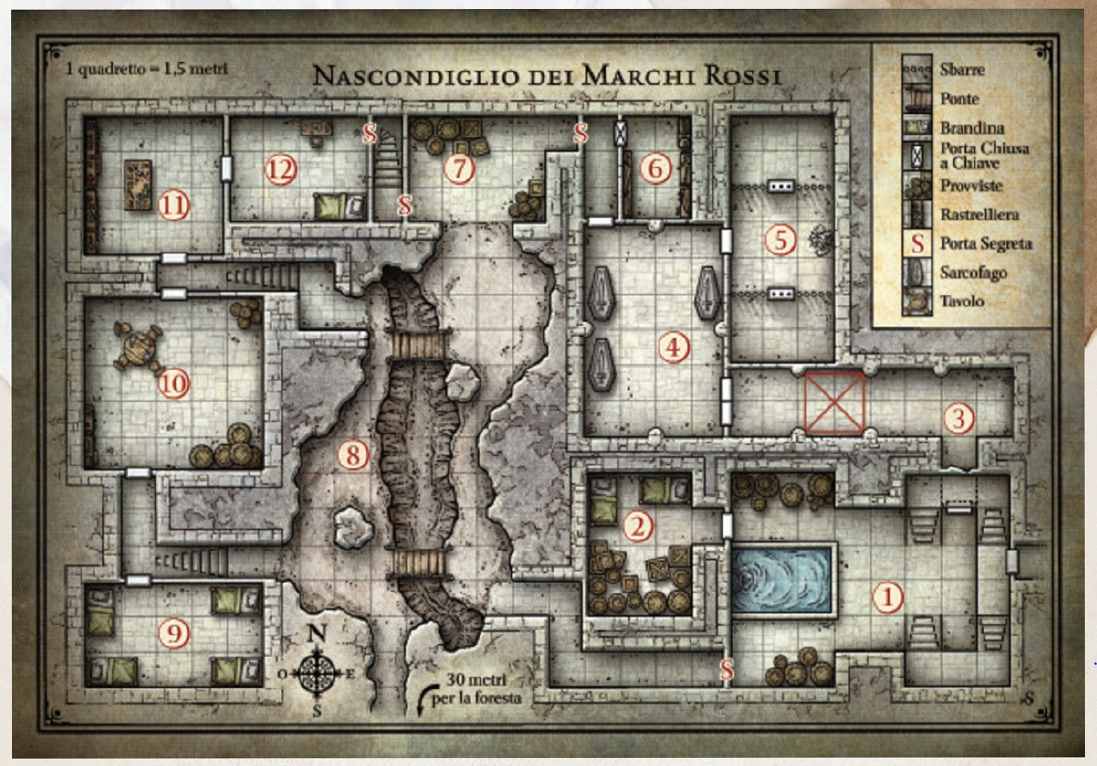
\includegraphics[width=20cm,height=12cm]{../Mappe/NascondiglioDeiMarchiRossi.PNG}
\end{figure}


    \subparagraph{Cantina} Un’esplorazione del maniero rivela che l’edificio è deserto,
    ma ci sono numerose tracce che conducono a una scalinata
    di pietra situata accanto alle rovine di una grossa cucina. In
    fondo alla scala è visibile una porta che si affaccia su una
    cantina. La porta non è chiusa a chiave.
    Quando i personaggi la aprono, il DM legge il brano seguente:
        \begin{itemize}
                    \item \textbf{Descrizione}\textsc{La porta si apre su un pianerottolo largo un metro e mezzo che si
                affaccia su una grossa cantina ad almeno quattro metri e mezzo
                di altezza, con due brevi rampe di scalini di pietra che scendono
                fino al pavimento. Un'altra porta è situata sotto le scale a nord.
                Una grossa cisterna di pietra occupa la parte occidentale della
                stanza, lungo le cui pareti sono allineati barili e barilotti.}
                            \item Questa stanza sembra essere una grande cantina
                sotterranea, esattamente come quella che ci si aspetterebbe
                di trovare sotto un vecchio maniero. I Marchi Rossi vogliono
                tenere nascosto il loro quartier generale, quindi ad eccezione
                dei barili pieni di provviste fresche, nulla in questa stanza
                tradisce la loro presenza.
                I barili contengono maiale e manzo salato, farina,
                zucchero, mele e birra. Spostare i barili per esaminarli
                meticolosamente è un'attività rumorosa che attira l’attenzione
                dei Marchi Rossi nell’area 2
                        \begin{enumerate}
                            \item \textbf{Cisterna}Questa riserva rettangolare è pulita e piena di
                        acqua fredda potabile. È profonda 3 metri e ha un bordo
                        rialzato di 60 centimetri rispetto al resto del pavimento
                        (quindi il fondo della cisterna si trova a 2,4 metri di profondità
                        rispetto al pavimento). I tubi di scolo che partono dal tetto del
                        vecchio maniero riforniscono la cisterna di acqua.
                        Una sacca impermeabile è appesa a una corda sommersa
                        attaccata alla parete sud della cisterna, a circa 60 centimetri
                        sotto la superficie dell’acqua. Da fuori dall'acqua non è
                        visibile, ma può essere trovata effettuando con successo una
                        prova di Saggezza (Percezione) con CD 15 o automaticamente
                        se un personaggio sonda la cisterna con un'asta o vi salta
                        dentro. La sacca contiene alcuni oggetti preziosi (vedi la
                        sezione “Tesoro”).
                        \item \textbf{Porta Segreta}Una porta segreta è situata all'angolo
                        sudovest della stanza. Vedi la sezione “\hyperlink{trattigen}{Tratti Generali}” per
                        ulteriori informazioni sulle porte segrete.
                                \end{enumerate}
                        \item \textbf{Sviluppi} Nessun mostro o nemico è presente in quest'area, ma
                        i malviventi dell’area 2 si accorgeranno della presenza
                        dei personaggi, se questi fanno molto rumore quaggiù. I
                        malviventi entrano nella stanza di soppiatto e beneficiano
                        di sorpresa se i personaggi non li sentono (vedi “Sorpresa”
                        nel regolamento). Se i malviventi combattono in quest'area
                        e due di loro vengono sconfitti, l’ultimo potrebbe rivelare la
                        presenza della porta segreta fuggendo in quella direzione.

                        \item \textbf{Tesoro} La sacca nascosta nella cisterna è impermeabile e contiene
                        una pozione di guarigione, una pozione di invisibilità, 50 mo
                        e semplici abiti da viaggio puliti. Si tratta di un kit di fuga che
                        Tarno ha nascosto quaggiù in caso di emergenza.
                        \end{itemize}
    
    \subparagraph{Dormitorio} 
        Buona parte dei membri umani dei Marchi Rossi alloggia
    aa Phandalin. Questo dormitorio è un buon posto dove far
    calmare le acque dopo un'incursione ai danni dei minatori e
    dei mercanti di pellicce locali. Tre malviventi dei Marchi Rossi riposano in questa stanza.
    Se sentono molto rumore nell’area 1 (come qualcuno che
    parla a voce alta o un barile che viene fatto rotolare), si
    preparano a combattere e tentano di sorprendere gli intrusi.
    I barili di questa stanza contengono scorte simili a
    quelle dell’area 1.

        \textbf{Descrizione Area 2} \\ Questo sembra essere un magazzino riadattato ad alloggio
        temporaneo. Due letti a castello sono stati sistemati lungo la
        parete accanto alla porta, mentre la parte sud della camera è
        occupata da casse e barili.\\
        \textbf{Tesoro} Ognuno dei tre Marchi Rossi porta alla cintura una borsa
        che contiene un piccolo tesoro. Il primo possiede 16 ma e 7
        mo, il secondo 12 ma e 5 mo e il terzo 15 me e due granati
        (10 mo ciascuno). Inoltre, tre sporchi mantelli scarlatti sono
        appesi ai letti.


            \subparagraph{Corridoio con Trappola} Quest'area faceva parte delle cantine originali del Maniero
            Tresendar. I Marchi Rossi hanno scavato e rimosso il
            terriccio sotto il pavimento di pietra, creando una fossa
            nascosta che usano come trappola.La fossa nascosta al centro del corridoio è celata sotto un
            falso pavimento fatto di pietre lastricate non cementate
            disposte su una fila di fragili assi di legno. Le pietre e le assi
            crollano sotto un peso pari o superiore a 50 chilogrammi. Se
            un personaggio cerca trappole nel corridoio, riesce a notare la
            fossa nascosta superando una prova di Saggezza (Percezione)
            con CD 15. Una prova effettuata con successo rivela anche
            degli esili cornicioni che corrono sul lato sud e sul lato nord
            della fossa. Una creatura può tentare di sgusciare oltre la
            fossa passando su uno di quei cornicioni ed effettuando con
            successo una prova di Destrezza (Acrobazia) con CD 10.
            Se una creatura innesca la trappola o fallisce la prova
            di Destrezza per sgusciare lungo il bordo della fossa, deve
            superare un tiro salvezza su Destrezza con CD 15 per
            ‘aggrapparsi al bordo. In caso di fallimento, la creatura cade
            per 6 metri sul pavimento di terriccio della fossa, subisce 2d6
            danni contundenti e atterra prona.\\
            \textbf{Descrizione area 3} Un fitto strato di polvere ricopre le pietre lastricate di questo cupo corridoio. Le pareti sono decorate con finte colonne
            disposte a intervalli di tre metri e la doppia porta all'estremità
            ovest del corridoio è rivestita di una placcatura in rame che col
            passare del tempo è diventata verde. La porta è decorata con
            un bassorilievo che raffigura un angelo piangente. (100 PE per la trappola)\\


        \subparagraph{Cripte Di Tresendar}
                Gli antenati della famiglia Tresendar, ormai scomparsa da
        tempo, venivano un tempo sepolti in questo mausoleo. I tre scheletri sono animati e attaccano qualsiasi creatura
        che giunga entro 3 metri dalla porta che conduce all'area 5 0
        quella che conduce all’area 6, a meno che quella creatura non
        indossi il mantello scarlatto dei Marchi Rossi o non pronunci
        la parola d'ordine “Illefarn” (il nome di un'antica nazione elfica
        che un tempo occupava buona parte della Costa della Spada).
        Il coperchio di pietra di ogni sarcofago è scolpito in modo
        da raffigurare il defunto all’interno (due maschi umani e una
        femmina umana, tutti di portamento nobiliare). Se aperte, le
        tombe rivelano soltanto un cumulo di ossa ammuffite e alcuni
        brandelli di abiti, ma vedi la sezione “Tesoro”.\\
                \textbf{Descrizione: }Questa cripta polverosa ospita tre grossi sarcofagi di pietra,
        su ognuno dei quali poggia uno scheletro umano vestito di
        frammenti arrugginiti di una cotta di maglia. Le finte colonne
        lungo le pareti sono scolpite per assomigliare a querce dai
        rami protesi verso il soffitto. La doppia porta nell’angolo
        sudest è rivestita di una consunta placcatura in rame.\\
        \textbf{Sviluppi: }Un combattimento in questa stanza mette in allarme i Marchi
        Rossi nell’area 5.\\
        \textbf{Tesoro: }Tra le ossa di ogni sarcofago è nascosto un anello con sigillo
        in platino (50 mo).

        \subparagraph{Recinti Degli Schiavi} Negli ultimi due mesi i Marchi Rossi hanno catturato vari
        viaggiatori che attraversavano l’area e li hanno rinchiusi in
        questi recinti, in attesa di poterli vendere come schiavi. Due malviventi dei Marchi Rossi nei loro mantelli scarlatti
        montano la guardia in quest'area, anche se passano buona
        parte del loro tempo a tormentare i prigionieri inermi (vedi
        la sezione “Prigionieri”). Se sentono combattere nell’area
        4, prendono posizione contro la parete accanto alla porta,
        nel tentativo di sorprendere gli intrusi. I prigionieri sono
        troppo intimoriti per lanciare un grido di avvertimento o
        chiedere aiuto. Gli abiti accumulati su un lato appartenevano ai vari
        prigionieri che sono stati rinchiusi quaggiù nel giro degli
        ultimi due mesi (almeno una dozzina di persone, a giudicare
        dalle dimensioni del cumulo).\\

        \textbf{Porte Delle Celle: } Le porte delle celle sono dotate di
        serrature semplici che possono essere scassinate usando gli
        arnesi da scasso ed effettuando con successo una prova di
        Destrezza con CD 10. Le porte possono anche essere sfondate
        usando la forza bruta, superando una prova di Forza con CD 22.\\

        \textbf{Descrizione: }Questa lunga stanza è suddivisa in tre aree ed è delimitata
        a norde a sud da una fila di sbarre di ferro. Il pavimento
        delle celle è ricoperto da un lercio strato di paglia e le porte
        montate su cardini sono bloccate da catene e lucchetti. Due
        donne dall’aspetto esausto sono rinchiuse nella cella a sud,
        mentre un ragazzino umano occupa la cella a nord. Tutti i
        prigionieri indossano semplici tuniche grigie e portano un
        collare di ferro al collo.
        Alcuni abiti scartati sono stati accumulati alla rinfusa contro la
        parete di fondo.\\

        \textbf{Prigionieri} I tre popolani umani imprigionati quaggiù sono Mirna Dendrar
        ei suoi due figli, Nars di tredici anni e Nilsa di diciotto anni.
        Alcuni giorni fai Marchi Rossi hanno assassinato il marito di
        Mirna, Thel, che aveva osato tenere testa ai malviventi. (Il suo
        cadavere si trova nell’area 8.) Quella notte la banda ha fatto
        ritorno in paese e ha rapito la famiglia dalla sua abitazione di
        Phandalin, con l'intenzione di venderla in schiavitù.
        I Dendrar sono grati ai personaggi per il salvataggio, ma
        non hanno molte informazioni da fornire sul nascondiglio dei
        Marchi Rossi. Sanno solo che il loro capo è un mago (anche
        se non l'hanno mai incontrato e non conoscono il suo nome) e
        che tiene alcuni “mostri alti e pelosi dalle grandi orecchie” (i
        bugbear) al suo servizio. \\

        \textbf{Missione Secondaria: Il Cimelio di Mirna.} Anche se la
        sua famiglia non ha niente da offrire come ricompensa, Mirna
        rivela ai personaggi che potrebbe sapere dove è custodito
        un prezioso cimelio. Quando era ancora una ragazzina, la
        sua famiglia fuggì da Thundertree a causa dell'invasione dei
        non morti. La sua famiglia possedeva una bottega di erbe
        e alchimia, e nel negozio c'era una custodia che conteneva
        una collana di smeraldo, nascosta dietro uno scaffale del
        magazzino. Non ha mai avuto il coraggio di tornare laggiù
        per recuperarla. Il negozio si trovava nella zona sudest di
        Thundertree. Se i personaggi decidono di esplorare le rovine
        di Thundertree, vedi la terza parte dell’avventura.
 
        \subparagraph{Armeria} La porta di questa stanza è chiusa a chiave dall’esterno. Di
    fronte alla porta chiusa c'è una porta segreta che conduce
    all'area 7. Per ulteriori informazioni sulle porte chiuse e sulle
    porte segrete, vedi la sezione “\hyperlink{trattigen}{Tratti Generali}” I Marchi Rossi sono ambiziosi e intendono ampliare le loro
    attività nell'immediato futuro, quindi hanno iniziato ad
    accumulare armi e armature.
    Le rastrelliere per armi contengono dodici lance, sei spade
    corte, quattro spade lunghe, sei balestre leggere e otto faretre
    contenenti venti quadrelli da balestra ciascuna.\\
        
        \textbf{Descrizione:} Lungo le pareti di questa camera sono appoggiate varie
    rastrelliere cariche di armi come lance, spade, balestre e
    quadrelli. Su un attaccapanni accanto alla porta sono appesi
    circa una dozzina di sporchi mantelli rossi.

    \subparagraph{Magazzino e Officina} I Marchi Rossi hanno accumulato in questa camera le merci
    che hanno rubato. Da qui le spediscono a sud attraverso le
    caverne o le imballano per custodirle nella roccaforte. Questa stanza contiene due porte segrete, una che conduce
    all’area 6 e l’altra all'area 12. Vedi la sezione “\hyperlink{trattigen}{Tratti Generali}”
    (pagina 20) per ulteriori informazioni sulle porte segrete.\\

    \textbf{Descrizione:} Quest’area è costituita dalla parte nord di una grossa
    caverna naturale, rifinita con pareti in pietra lavorata e un
    pavimento lastricato. Lungo le pareti sono stati impilati vari
    barili, assieme a numerose casse vuote, cumuli di paglia da
    imballaggio, martelli, piedi di porco e chiodi.
    La caverna prosegue per una certa distanza verso sud. Riuscite
    a distinguere vari passaggi che si aprono lungo il tratto più
    ampio della caverna e quella che sembra una profonda fossa o
    un crepaccio che si apre sul pavimento.\\
    \textbf{Tesoro} Buona parte delle scorte e delle merci custodite in questa
    stanza non è di grande valore, ma in mezzo alle scorte ci
    sono trenta pellicce di castoro (2 mo ciascuna) saccheggiate
    da una carovana che procedeva lungo la Pista di Triboar
    alcuni giorni fa.
    \subparagraph{Crepaccio} I personaggi possono arrivare qui da tre direzioni diverse:
    dal tunnel dall'area 1, dal magazzino dall’area 7 o dal
    passaggio in pietra grezza a sud, che continua oltre la mappa
    per circa trenta metri fino a sfociare nei boschi a sud del
    Maniero Tresendar. Il passaggio è un modo eccellente per
    contrabbandare persone o merci dentro e fuori da Phandalin
    senza essere visti ed è una risorsa perfetta per una banda di
    ladri e schiavisti.
    Il guardiano della caverna è un nothic, un folle mostro
    sotterraneo affamato di carne. La creatura, attirata da un
    debole effetto magico emanato dal crepaccio, occupava l'area
    fin da prima che i Marchi Rossi si stabilissero sul posto. Iarno
    é riuscito a stringere un accordo con il mostro, convincendolo
    a sorvegliare la roccaforte in cambio di tesori e di qualche
    dose di carne fresca di tanto in tanto. Tuttavia, del nothic non
    ci si può fidare.
    Il \hyperlink{nothic}{nothic} si annida nei pressi delle estremità ovest dei
    due ponti. Se nota degli intrusi nella caverna, si nasconde
    dietro una delle due grosse colonne di pietra e li osserva,
    tentando di usare la sua Intuizione Innaturale (vedi la scheda
    delle statistiche della creatura) per discernere i segreti
    dei personaggi.
    Il nothic comunica telepaticamente. Se viene scoperto,
    preferisce negoziare e non si fa troppi scrupoli a tradire
    i Marchi Rossi di fronte a un incentivo giusto, come una
    promessa di cibo. Interpretando il nothic, il DM dovrebbe
    parlare sussurrando e alternando alle parole qualche folle
    risatina e frase senza senso. Dovrà inoltre spiegare che
    la creatura non sta parlando: i suoi folli mormorii e le sue
    richieste di cibo echeggiano direttamente nella testa dei
    personaggi. Il nothic sa tutto ciò che sanno i Marchi Rossi;
    vedi il riquadro “\hyperlink{cosasanno}{Cosa Sanno i Marchi Rossi}”. \\
    \textbf{Frasi senza senzo del Nothic}\\
    \begin{itemize}
        \item \textit{"I tuoi segreti sono scritti nelle cicatrici della mia pelle."}
        \item \textit{"La mia fame per il potere non conosce limiti; tremate di fronte alla mia sete."}
        \item \textit{"Le urla dei dannati sono la mia musica preferita."}
        \item \textit{"I miei occhi vedono oltre il velo della tua falsa sicurezza."}
        \item \textit{"Le tue paure sono le corde che suono nel mio tormento."}
    \end{itemize}

    \textbf{I segreti dei PG}
    D10 per scegliere di chi scopre i segreti ( 1-2 Thia, 3-4 Bryseis, 5-6 Leandra, 7-8 Atalanta, 9 - 10 Kai)
    \begin{enumerate}
        \item Thia: membro di un'importante famiglia elfica di Evermeet
        \item Bryseis: \begin{enumerate}
            \item Se non hanno ancora parlato di Cassiopea: Odio verso gli umani ( La stuzzica dicendo che la sua razza dovrebbe essere sterminata)
            \item Se ne hanno parlato e non ha ancora ammesso che è colpa sua, rivela la sua colpa
            \item Parla del suo passato e da fatto di essere considerata un mostro
        \end{enumerate}
        \item Leandra: Incalza sul fatto di essere stata abbandonata
        \item Atalanta: genitori adottivi morti e abbandono.
        \item Kai: parla del suo odio represso
    \end{enumerate}
\textbf{Descrizione: }
\begin{itemize}
    \item \textbf{Ponti} Questi ponti sono fatti di assi di legno e sono privi
    di ringhiere. Il ponte sud è manomesso in modo da crollare se una creatura di peso superiore ai 25 chilogrammi lo
    attraversa. Un personaggio accanto al ponte può capire che la
    costruzione è difettosa superando una prova di Intelligenza
    (Indagare) con CD 15. Una creatura può usare un'azione per
    scalzare un supporto all'estremità di un ponte, facendolo
    precipitare nel crepaccio. 
    \item \textbf{Crepaccio} Questo crepaccio dalle pareti ripide è largo
    dagli 1,5 ai 3 metri ed è profondo 6 metri. Le sue pareti
    rocciose irregolari possono facilmente essere scalate senza
    dover effettuare alcuna prova di caratteristica. Se una
    creatura cade nel crepaccio, subisce 2d46 danni contundenti
    e atterra prona su uno strato di detriti considerato terreno
    difficile (vedi “Terreno Difficile” nel regolamento).
    Il fondo del crepaccio emana un freddo innaturale. Se
    esaminata attraverso un incantesimo individuazione del
    magico, l’area emana una debole aura necromantica. La
    magia rallenta l'invecchiamento e la decomposizione di tutta
    la materia organica a metà della velocità normale.
    Sul fondo del crepaccio, in mezzo a uno strato di ossa
    spolpate e rosicchiate, giace il cadavere semisbranato di
    Thel Dendrar, l'intagliatore ucciso dai Marchi Rossi. I
    fuorilegge hanno gettato quaggiù il cadavere affinché il nothic
    potesse cibarsene.
    \item \textbf{Tesoro}Il nothic custodisce il suo tesoro in un malconcio forziere di
    legno nascosto in un cunicolo in fondo al crepaccio, sotto il
    ponte nord. Il forziere non è visibile dai bordi del crepaccio,
    ma risulta evidente a qualsiasi personaggio che scenda sul
    fondo. Il forziere contiene 160 ma, 120 mo, cinque malachiti
    (gemme da 15 mo ciascuna), due pozioni di guarigione e una
    pergamena di presagio. Il forziere contiene anche una spada lunga +1 custodita in
    un fodero filigranato d’argento. Sulla spada è inciso il nome
    “Artiglio” e la sua impugnatura ha la forma di un rapace dalle
    ali spiegate. Un tempo apparteneva a un grande cavaliere
    di nome Aldith Tresendar, noto come il Falco Nero. Se un
    personaggio effettua con successo una prova di Intelligenza
    (Storia) con CD 15, riconosce la spada e ricorda la sua storia.
    Sir Aldith morì combattendo gli orchi che attaccarono il
    maniero sfruttando le caverne sotterranee. Artiglio andò
    perduta in quell’occasione, finché non fu ritrovata dal nothic.
    \item \textbf{Punti}I personaggi si dividono equamente 450 PE se sconfiggono il
                nothic o negoziano con lui una tregua.
\end{itemize}





        \subparagraph{Dormitorio delle guardie} Se un personaggio origlia a questa porta ed effettua con
        successo una prova di Saggezza (Percezione) con CD 10,
        sente alcune voci rauche che impartiscono dei comandi
        degradanti nel linguaggio dei Goblin, come per esempio
        “Lecca il pavimento!” e “Rotolati come un cane!” I bugbear in
        questa stanza si divertono a maltrattare il loro schiavo goblin.
        In quest'area sono presenti tre bugbear e un goblin. Il
        goblin, Droop, sviene non appena vede il gruppo, ma un’altra
        creatura può usare un’azione per risvegliarlo. Altrimenti,
        Droop resta privo di sensi per 1410 minuti.
        I bugbear lavorano perIl Divoratore di Luce e sono stati inviati
        quaggiù per aiutare larno a tenere in riga i Marchi Rossi e
        gli abitanti di Phandalin. Il capo dei bugbear si chiama Mosk
        e su un occhio porta una benda ingioiellata, anche se lo fa
        semplicemente perché gli piace, non certo per necessità.
        I bugbear evitano i membri umani dei Marchi Rossi. Se i
        personaggi indossano i mantelli scarlatti che hanno trovato
        in qualche altra area, i bugbear presumono che siano al
        servizio di Iarno. I personaggi più astuti potrebbero perfino
        persuadere i bugbear a occuparsi dei “traditori” o degli
        “impostori” che si trovano in un’altra parte del dungeon. Se
        il DM ritiene che i giocatori non se la stiano cavando troppo
        bene a mettere in scena questo inganno, può chiedere al
        personaggio che ha parlato più degli altri di effettuare una
        prova di Carisma (Inganno) con CD 15 per convincere i
        bugbear a fare cid che il gruppo vuole. \\
        \textbf{Descrizione: } Questo dormitorio contiene quattro brandine di legno
        rozzamente costruite, circondate da cumuli di coperte e
        piatti sporchi sparsi in giro per la stanza. Laria é satura della
        puzza di corpi sporchi e di carne putrefatta. Tre umanoidi alti
        e pelosi se ne stanno seduti in mezzo al disordine, urlando
        ordini a un triste e piccolo goblin che si umilia per divertirli.
        Alla vostra improvvisa apparizione, il goblin sviene.\\
        \textbf{Droop} Il goblin Droop non è una minaccia per il gruppo. I bugbear
        fanno i prepotenti con lui e lo costringono a obbedire ai loro
        ordini, almeno finché non si fa avanti qualcuno di più forte.
        Se riprende conoscenza durante il combattimento, Droop
        si nasconde ed evita lo scontro. È talmente codardo che se gli
        viene ordinato di combattere, lo fa subendo svantaggio (come
        spiegato nel regolamento).
        Droop conosce la disposizione generale delle stanze nel
        nascondiglio dei Marchi Rossi, nonché l’ubicazione delle
        trappole e delle porte segrete. Non pensa di sua iniziativa a
        fornire queste informazioni, ma se gli viene chiesto, rivela
        tutto ciò che riesce a ricordare nel tentativo di essere utile al gruppo. Alcuni dettagli, tuttavia, potrebbero risultare confusi
        o mescolati. Dopotutto è pur sempre un goblin.
        Se i bugbear vengono eliminati, Droop tenta di entrare
        nelle grazie del gruppo. Non ricorda la strada per il Castello
        Cragmaw, ma sa che si trova a nord, in una foresta. Sa anche
        che i goblin Cragmaw pattugliano i dintorni di Phandalin
        e suggerisce ai personaggi di catturare una pattuglia per
        ottenere più informazioni sul castello.
        I personaggi potrebbero decidere di tenere Droop con
        loro per un po’. Vedi il riquadro “PNG Membri del Gruppo”
        (pagina 11) per alcuni consigli su come gestire Droop
        facendone un membro del gruppo.
        \textbf{Sviluppi} I bugbear sono gli unici nel nascondiglio dei Marchi Rossi
        a sapere dove si trova la Caverna dell’Onda Tonante. Non
        divulgheranno questa informazione, dal momento che temono
        L'Oscuro ben più dei personaggi
        I bugbear sanno anche dove si trova il Castello Cragmaw,
        ma non condivideranno questa informazione volontariamente.
        Se un personaggio interroga un bugberar catturato, può
        strappargli queste informazioni effettuando con successo una
        prova di Carisma (Intimidire) con CD 15.
        Mosk porta alla cintura una borsa che contiene 33 ma
        e indossa una benda per l’occhio fatta di cuoio nero e
        incastonata di gemme semipreziose (50 mo). Possiede inoltre
        una chiave di ferro che può aprire e chiudere tutte le porte del
        nascondiglio dei Marchi Rossi.\\
        \textbf{Tesoro}
        Mosk porta alla cintura una borsa che contiene 33 ma
        e indossa una benda per l’occhio fatta di cuoio nero e
        incastonata di gemme semipreziose (50 mo). Possiede inoltre
        una chiave di ferro che può aprire e chiudere tutte le porte del
        nascondiglio dei Marchi Rossi.
        \subparagraph{Sala Comune} 
        Quest'area funge da quartier generale e sala riunioni dei
        Marchi Rossi. Quando non c'è alcuna questione ufficiale
        da discutere, funge anche da sala comune dove le guardie
        della roccaforte possono rilassarsi nelle ore in cui non
        sono in servizio.
        Se un personaggio origlia alla porta effettuando una prova
        di Saggezza (Percezione) con CD 10, sente chei nemici
        all’interno sono impegnati in una partita di aliossi. Questo
        genera un misterioso rumore tamburellante, seguito da varie
        grida e gemiti e da un improvviso brusio di voci che parlano
        di scommesse da pagare. Se i personaggi fanno irruzione
        nella stanza, sorprendono automaticamente i suoi occupanti. Quattro malviventi dei Marchi Rossi bevono e giocano ad
        aliossi quando i personaggi entrano. La partita è in procinto
        di degenerare, come capita spesso. I dadi sono truccati e
        il malvivente che li possiede, naturalmente, sta vincendo.
        Tutti e quattro hanno bevuto parecchio e sono considerati
        avvelenati (vedi l’appendice del regolamento per gli effetti
        della condizione di avvelenato). I Marchi Rossi riconoscono immediatamente come
        impostori gli eventuali personaggi che indossano un mantello
        scarlatto. Tuttavia, un personaggio con una buona parlantina
        potrebbe riuscire a spacciare lui e i suoi compagni per “nuove
        reclute”, specialmente se si offre di unirsi alla partita. Se il
        DM ritiene che i giocatori non se la stiano cavando troppo
        bene a interpretare l'inganno, può chiedere al personaggio
        che ha parlato di più di effettuare una prova di Carisma
        (Inganno) con CD 10 per imbrogliare i Marchi Rossi. 
        \textbf{Descrizione:} Alcuni vecchi tavoli e sedie sono sparpagliati in giro per questa
        vasta stanza. Lungo le pareti, decorate da tende rosse e marroni,
        sono state allineate alcune panche di legno e vari barilotti di birra
        sono stati piazzati su un tavolo e dotati di una spina.
        Quattro combattenti umani di solida stazza che indossano
        mantelli scarlatti siedono attorno a uno dei tavoli. Un cumulo di
        monete e di monili è visibile al centro del tavolo.\\
        \textbf{Tesore:} Le ricchezze di questa stanza sono tutte visibili sul tavolo,
        dal momento che sono state usate come posta della partita.
        (Rovesciare il tavolo o mescolare il bottino dei nemici è
        un ottimo modo per distrarli temporaneamente.) Il totale
        ammonta a 75 mr, 55 ma, 22 me, 15 mo e un paio di orecchini
        d’oro con un minuscolo rubino incastonato (30 mo).\\

        \subparagraph{Laboratorio del mago} Da oltre le porte di questa stanza è possibile sentire il rumore
di qualcosa che bolle e che gocciola effettuando con successo
una prova di Saggezza (Percezione) con CD 15. Tarno ha lasciato qui il suo topo famiglio a fare la guardia in
caso di intrusi. Il topo condivide un legame telepatico con il
padrone e invia un breve messaggio d’avvertimento a Iarno
non appena vede gli intrusi. Il topo si muove a una velocità di
6 metri e ha CA 10, 1 punto ferita e nessun attacco efficace.
Se il topo viene ucciso, scompare.
Se i personaggi lo lasciano stare, il topo li segue per il resto
del dungeon, come se fosse curioso o affamato. Potrebbe
perfino fingere di provare affetto per un personaggio
che gli dia da mangiare, ma in realtà resta fedele fino in
fondo a Jarno. \\
\textbf{Libri e Appunti} larno sta cercando di apprendere l’arte
di mescere pozioni e fabbricare misture alchemiche. I libri e
gli appunti sparpagliati per la stanza sono testi di alchimia
elementare. Qualsiasi personaggio competente in Arcano può
capire che l’apparecchiatura di larno sembra predisposta per
mescere pozioni di invisibilità... anche se finora non sembra
esserci riuscito.
Tra i libri c'è un tomo scritto in Nanico: si tratta del
diario di un avventuriero di nome Urmon e narra la
storia della Miniera Perduta di Phandelver e della Forgia
degli Incantesimi. (Il DM condivide coni giocatori le
informazioni del primo e del secondo paragrafo della
sezione “Background”, se non lo ha già fatto.) Inoltre, Urmon
parla di una mazza magica chiamata Portatrice di Luce,
commissionata dai sacerdoti di Lathander, il dio dell’alba, ai
maghi che lavoravano assieme agli gnomi e ai nani del Patto
di Phandelver. La mazza andò perduta quando la Caverna
dell’Onda Tonante e la sua miniera scomparvero dalla storia.
(I personaggi potrebbero ritrovare la mazza nella quarta
parte, “La Caverna dell’Onda Tonante”.)\\
\textbf{Descrizione:} Questa stanza sembra essere il laboratorio di un mago. Un
topo zampetta sul pavimento per rifugiarsi sotto un grosso
tavolo da lavoro carico di storte, alambicchi, serpentine da
distillazione e altri strumenti alchemici, tutti pieni di sostanze
messe a scaldare che gorgogliano costantemente. Le mensole
sono piene di rotoli di pergamene e di tomi dall’aspetto strano.\\
\textbf{Sviluppi:} Dal momento che Iarno e il suo topo famiglio condividono un
legame telepatico, il mago (nell’area 12) sa che i personaggi
stanno arrivando e ha tempo di prepararsi ad affrontarli.\\
\textbf{Tesoro:} La maggior parte del materiale contenuto in questa stanza
è privo di valore, ma tre bottigliette contengono dei reagenti
rari: mercurio, bile di drago e belladonna in polvere. Ognuna
vale 25 mo se venduta a uno speziale o a un alchimista.
\subparagraph{Alloggi di Bastone di vetro} Se i personaggi raggiungono questa stanza dal passaggio
segreto dell'area 7, possono cogliere di sorpresa il capo dei
Marchi Rossi, Iarno “Bastone di Vetro” Albrek. Altrimenti
il suo topo famiglio lo avverte di chiunque passi attraverso
l’area 11 e il mago fugge prima che i personaggi arrivino. \\
 \textbf{Descrizione} \textsc{ Le pareti di questa camera da letto sono ricoperte di drappi
scarlatti. La mobilia include una piccola scrivania, una sedia,
un comodo letto e un forziere di legno ai piedi del letto. }
\textit{Se Iarno è stato sorpreso, il DM aggiunge il
paragrafo seguente.} \textsc{Un basso umano dalla barba nera e vestito con un'ampia
tunica siede alla scrivania, intento a studiare un tomo. Indossa
uno sfarzoso mantello di ermellino. Tiene a portata di mano
un magnifico bastone di vetro appoggiato alla sedia.}
Se il topo nell’area 11 avverte il mago malvagio che ci
sono guai in arrivo, larno prende il suo bastone di difesa
(vedi l’appendice A) e le pergamene nel suo forziere (vedi
la sezione “Tesoro”), per poi fuggire attraverso la porta
segreta situata nell'angolo nordest della stanza. Nella fretta,
Jarno dimentica nella stanza una lettera del Ragno Nero
(vedi la sezione “Sviluppi”) e non richiude completamente
la porta segreta. I personaggi dispongono di vantaggio alle
prove di caratteristica effettuate per notare la porta segreta
leggermente socchiusa (vedi “Vantaggio e Svantaggio” nel
regolamento). Per ulteriori informazioni sulle porte segrete,
vedi la sezione “Tratti Generali” (pagina 20).
Se riesce a fuggire, Iarno raggiunge l’area 1 (attraverso
le aree 7 e 8) e afferra la sacca nascosta nella cisterna di
quell’area. Se il nothic dell’area 8 è ancora vivo, Iarno gli
ordina di intercettare gli inseguitori. Se i personaggi lo
raggiungono, larno beve la pozione di invisibilità nascosta
nella sacca e fugge dal nascondiglio. A discrezione del
DM, potrebbe ricomparire successivamente nel corso
dell'avventura.

\textbf{Iarno:}Iarno è un ex-membro dell'Alleanza dei Lord che, una volta
giunto a Phandalin, ha colto un'opportunità per arricchirsi.
In origine il mago aveva l’incarico di fondare una forza
di vigilanza, ma decise invece di radunare un gruppo di
fuorilegge e di malviventi locali per assicurarsi una posizione
privilegiata in paese.
larno sapeva dell'esistenza del Ragno Nero grazie ai suoi
contatti nell’Alleanza dei Lord e ottenne un incontro con lui.
Il drow promise di condividere i segreti e le ricchezze della
Forgia degli Incantesimi con il mago in cambio del suo aiuto e
della sua lealtà.
Tarno mantiene un atteggiamento
elegante e cortese, rivolgendosi ai
malviventi con l'appellativo di “miei
cari signori” e riferendosi agli atti più
sordidi come i rapimenti e gli incendi
definendoli “quello spiacevole piccolo
affare” o “quella sfortunata tragedia”.
Si rivolge ai personaggi chiamandoli
“ospiti” e si scusa per non aver fornito loro
un intrattenimento adatto in occasione
di questa visita. Dietro questa facciata
di cortesia, tuttavia, larno è spietato e
arrogante esattamente quanto i fuorilegge
dei Marchi Rossi.
Se minacciato, larno usa il suo bastone
di difesa per lanciare armatura magica su
se stesso, poi lancia alcuni incantesimi
offensivi sui nemici che è in grado di
vedere. La scheda delle statistiche di larno
contiene la lista degli incantesimi che ha
preparato. Per le descrizioni e gli effetti
di quegli incantesimi, vedi il regolamento.
larno usa il potere scudo del suo bastone
per incrementare le sue protezioni.
Se scende a 8 punti ferita o meno e
non gli resta nessuna via di fuga, larno
si arrende. Considera la sua vita più
preziosa di qualsiasi cosa e si comporta
da prigioniero modello, nella speranza che
L'Oscuro venga a sapere in qualche
modo della sua situazione e “organizzi la
sua liberazione”. Se interrogato mentre è prigioniero,
Iarno rivela le informazioni seguenti, che
sono tutte vere:
\begin{itemize}
    \item Il Divoratore di Luce è un drow (un elfo
oscuro).
    \item Il Divoratore di Luce ha inviato tre bugbear per
aiutare larno a tenere la popolazione di
Phandalin sotto controllo, mai Marchi
Rossi se la sono cavata anche senza di
loro. I bugbear conoscono la strada che
porta alla Caverna dell’Onda Tonante,
mentre larno non la conosce.
    \item Il Divoratore di Luce è alla ricerca della
Caverna dell’Onda Tonante per
impadronirsi della Forgia degli
Incantesimi. I nani e gli gnomi del Patto
di Phandelver usavano la forgia magica
per fabbricare potenti oggetti magici.
    \item Nessun altro membro dell'Alleanza dei
Lord è al corrente del tradimento di
Tarno.
\end{itemize}
\textbf{Sviluppi:}
Vari documenti e appunti sono impilati ordinatamente sulla
scrivania. Si tratta per buona parte di ordini scritti che
Iarno intende spedire agli speziali e agli alchimisti degli
insediamenti vicini per ulteriori materiali da aggiungere
al suo laboratorio. I personaggi trovano anche una lettera
firmata con il simbolo del Ragno Nero. \textbf{LETTERA} \textsc{Lord Albrek,
Le mie spie a Neverwinter mi informano che presto
arriveranno alcuni stranieri a Phandalin. Potrebbero lavorare
peri nani. Catturali se puoi, uccidili se devi, ma non
permettere che interferiscano nei nostri piani. Assicurati
che ogni eventuale mappa nanica in loro possesso mi sia
consegnata rapidamente.
Conto su di te, larno. Non deludermi.}
Se Iarno viene messo sotto custodia, Sildar Hallwinter fa in
modo che il mago sia incarcerato nella villa del borgomastro
finché non potrà essere trasferito senza rischi a Neverwinter.
Se larno affronta o meno il processo per i suoi crimini è
qualcosa che va oltre la portata di questa avventura. Il Ragno
Nero ha troppo da fare per interferire nel destino del mago.

\textbf{Tesoro::}
AI piedi del letto di Iarno c'è un solido forziere di legno che
non è chiuso a chiave e che contiene le parti migliori dei
bottini che i Marchi Rossi hanno accumulato negli ultimi
due mesi. Il forziere contiene 180 ma, 130 mo e un sacchetto
di seta contenente cinque cornioli (10 mo ciascuno), due
peridotiti (15 mo ciascuna) e una perla (100 mo). Contiene
anche due oggetti magici che Iarno ha portato con sé da
Neverwinter: una pergamena di charme su persone e una
pergamena di palla di fuoco.
larno possiede inoltre un bastone di difesa (vedi
l’appendice A).

 

\subsection{Guest}
\subsubsection{CONYBERRY E LA TANA DI
AGATHA}
    \subparagraph{Viaggio} \begin{enumerate}
        \item Giorni di Viaggio: 3
        \item Giorno 1
                \begin{enumerate}
                    \item Tiro Nemici Diurni: 5 (Nessun nemico)
                    \item Tiro Nemici Notturni: 10 (Nessun nemico)
                \end{enumerate}
         \item Giorno 2
                \begin{enumerate}
                    \item Tiro Nemici Diurni: 7 (Nessun nemico)
                    \item Tiro Nemici Notturni: 14 (Nessun nemico)
                \end{enumerate}
         \item Giorno 3
                \begin{enumerate}
                    \item Tiro Nemici Diurni: 3 (Nessun nemico)
                    \item Tiro Nemici Notturni: 15 (Nessun nemico)
                \end{enumerate}
    \end{enumerate}
    \subparagraph{Descrizione per Agatha}Il paese di Conyberry fu saccheggiato dai barbari molti anni
fa e ora giace in rovina. La Pista di Triboar passa proprio
attraverso il paese abbandonato e costituisce un facile punto
di riferimento per individuare la tana della banshee Agatha.
Dalle rovine di Conyberry parte un vecchio sentiero che si
dirige a nordovest, addentrandosi nel Bosco di Neverwinter.
La tana di Agatha si trova ad alcuni chilometri fuori città.
\textsc{Il sentiero si addentra nel fitto degli alberi e la foresta si fa
più buia e impervia. Rampicanti aggrovigliati e folti strati di
muschio pendono dai rami e l’aria è palesemente più fredda
rispetto al villaggio in rovina. Dopo una curva lungo il sentiero,
notate una barriera fatta di rami deformi e fusi assieme fino a
creare un riparo a forma di cupola immerso nell'oscurità. Una
piccola porta consente di accedere all’interno.}
Se i personaggi si muovono con prudenza e ricordano perché
sono venuti, saranno in grado di parlare con la banshee.
Quando i personaggi entrano nel rifugio, il DM legge il
brano seguente: \textsc{Un’abitazione di qualche tipo è stata allestita all’interno
della cupola di rami intrecciati. È arredata con alcuni bauli,
mensole, un tavolo e una poltrona reclinata. Tutti i mobili
sembrano molto vecchi e di fattura elfica.}
Agatha percepisce l’intrusione dei personaggi e si manifesta
poco dopo il loro ingresso in casa sua. \textsc{Varia si fa gelida e siete colti da un'improvvisa sensazione di
terrore. Una luce fredda e pallida compare tremolando nell'aria
e assume rapidamente la forma di un'elfa la cui lunga chioma e
la tunica sono agitate da un vento spettrale. Forse un tempo era
di splendido aspetto, ma ora i suoi lineamenti sono deformati
da un'espressione di odio. “Stolti mortali”, ringhia. “Cosa vi ha
portato qui? Non sapete che cercarmi equivale alla morte?”}

    \subparagraph{Comportamento dei personaggi}
    \begin{itemize}
        \item Se i personaggi si comportano in modo scortese, irrispettoso
o minaccioso, Agatha si rabbuia e scompare. Non li
attacca, ma non fa ritorno nemmeno se i personaggi la
chiamano a lungo.
        \item Se i personaggi sono rispettosi e cortesi, Agatha può essere
persuasa ad aiutarli effettuando con successo una prova di
Carisma (Persuasione) con CD 15. Sarà il personaggio che
ha condotto principalmente le trattative a effettuare la prova.
Se il suo giocatore ha interpretato bene l’incontro, il DM
può consentirgli di effettuare la prova con vantaggio. Se un
personaggio è in possesso del pettine d’argento di Sorella Garaele e lo offre in dono ad Agatha, la prova ha successo
automaticamente. \textsc{La figura spettrale sorride sprezzante e sembra quasi divertita.
“Molto bene”, risponde. “So che cercate molte cose. Ponetemi
una singola domanda e io vi darò una risposta.”}Se i personaggi le chiedono del libro degli incantesimi di
Bowgentle, Agatha risponde di avere ceduto il libro a un
necromante di nome Tsernoth, proveniente dalla città di
Iriaebor oltre cento anni fa. Non sa che fine abbia fatto
poi il libro. La sua risposta è sincera ed è sufficiente a
Sorella Garaele per consentire agli Arpisti di riprendere le
loro ricerche.
I personaggi potrebbero invece decidere di porre ad Agatha
altre domande, come per esempio l'ubicazione del Castello
Cragmaw, l'ubicazione della Caverna dell’Onda Tonante,
l'identità del Ragno Nero o la domanda di Hamun Kost
riguardo al Pozzo del Vecchio Gufo (vedi quella sezione).
Agatha è bene informata ed è un’abile divinatrice, quindi può
rispondere praticamente a una qualsiasi domanda relativa
all'avventura che i personaggi decidano di porle. Tuttavia, la
banshee risponderà a una sola domanda, quindi i personaggi
dovranno scegliere saggiamente.
    \end{itemize}

\subparagraph{PE}I personaggi guadagnano punti esperienza se riescono a
convincere Agatha a rispondere a una domanda. In quel caso
si dividono equamente 200 PE.

\subsubsection{IL Pozzo DEL VECCHIO GUFO}
 \subparagraph{Viaggio} \begin{enumerate}
        \item Giorni di Viaggio: 3
        \item Giorno 1
                \begin{enumerate}
                    \item Tiro Nemici Diurni: 10 (Nessun nemico)
                    \item Tiro Nemici Notturni: 9 (Nessun nemico)
                \end{enumerate}
         \item Giorno 2
                \begin{enumerate}
                    \item Tiro Nemici Diurni: 1 (Nessun nemico)
                    \item Tiro Nemici Notturni: 15 (Nessun nemico)
                \end{enumerate}
         \item Giorno 3
                \begin{enumerate}
                    \item Tiro Nemici Diurni: 6 (Nessun nemico)
                    \item Tiro Nemici Notturni: 19 (Nemici: 4 Uccelli Stigei)
                \end{enumerate}
    \end{enumerate}
\subparagraph{Descrizione}
Il Pozzo del Vecchio Gufo, costruito migliaia di anni fa da
un impero scomparso da tempo, è una torre di guardia in
rovina costituita da poco più di alcune mura di cinta diroccate
e dal troncone infranto di una torre. Nel cortile della torre
c'è un vecchio pozzo che fornisce ancora oggi acqua fresca
e pulita. Il Pozzo del Vecchio Gufo si trova sulle colline
scoscese e selvagge a sud della Pista di Triboar. È un’area
relativamente facile da trovare e qualsiasi PNG di Phandalin
può fornire ai personaggi le indicazioni necessarie per
raggiungere le rovine.
Di recente alcuni cercatori minerari nell’area hanno notato
che qualcuno ha allestito un accampamento al Pozzo del
Vecchio Gufo e che alcuni guardiani non morti sono comparsi
con il compito di tenere alla larga gli intrusi.
\textsc{Una volta superato un basso crinale, avvistate le rovine di
una vecchia torre di guardia che si erge tra le colline scoscese.
È un luogo talmente antico che le mura di cinta ormai sono
soltanto cumuli di detriti che circondano una specie di cortile
adiacente al troncone diroccato di una vecchia torre. Una
tenda dai colori sgargianti è stata montata in mezzo al cortile,
ma non c'è nessuno in vista.}
a setacciare l’area nella speranza di recuperare conoscenze
arcane appartenenti ai suoi antichi costruttori. I personaggi
possono entrare nel complesso di rovine da qualsiasi
direzione, seguendo i vecchi sentieri o arrampicandosi
sul pendio e trovando un varco tra il muro di detriti
che lo circonda.
Dodici zombi si annidano tra le rovine della vecchia torre
di guardia e non sono visibili dall'esterno. Tuttavia, qualsiasi
personaggio con un punteggio di Saggezza (Percezione)
passiva di 10 o superiore percepisce un odore di putrefazione
che proviene dalla torre. Quando i personaggi si avvicinano
alla torre o alla tenda, gli zombi escono dalla torre a
passo strascicato.
Se ha inizio un combattimento, Hamun Kost, il mago
malvagio, esce dalla sua tenda e chiede: “Ma che significa
tutto questo?”
Kost è un individuo robusto che indossa una veste rossa.
Ha la pelle olivastra, il cranio rasato e un tatuaggio sulla
fronte. Se un personaggio effettua con successo una prova di
Intelligenza (Arcano) con CD 10 riconosce il tatuaggio di Kost
come un simbolo necromantico. Una prova di Intelligenza
(Storia) con CD 10 effettuata con successo rivela che le sue
vesti sono le tipiche vesti del Thay, una terra del lontano
est dove i maghi si coprono la pelle di tatuaggi. Il tatuaggio
sulla fronte rappresenta la scuola di magia a cui un mago
appartiene, che nel caso di Kost è la scuola di necromanzia.
Se un personaggio tenta di parlare con Kost, anche
invocando una tregua o rispondendo alle sue domande
durante il combattimento, Kost richiama temporaneamente i
suoi zombi. Il Mago Rosso non è particolarmente aggressivo
ed è disposto a stringere un accordo che torni a suo vantaggio
e che sia d'aiuto anche ai personaggi.
Kost tiene la bocca chiusa riguardo al motivo della sua
presenza nella regione, ma è disposto a fornire qualche
informazione di cui il gruppo ha bisogno, se in cambio
ottiene un favore. Se i personaggi forniscono a Kost qualche
indicazione su ciò che cercano, il mago condivide una o
entrambe le seguenti richieste:
\begin{itemize}
    \item Vuole che gli orchi al Tor della Viverna siano tolti di mezzo,
dal momento che hanno già avvistato il suo accampamento
e sembrano intenzionati a creare guai.
    \item Vuole porre una domanda ad Agatha la banshee: “Come si
chiama il mago che costruì la torre del Pozzo del Vecchio
Gufo?” Kost non vuole rischiare di suscitare la collera della
banshee, ma i personaggi potrebbero porre la domanda in
sua vece. (Agatha conosce la risposta: Arthindol.)
\end{itemize}

\subparagraph{Se sconfiggono Kost e gli zombie} possono entrare nella tenda e trovano : La tenda di Hamun Kost è arredata con una comoda
attrezzatura da viaggio che include una brandina, una sedia,
una scrivania, varie provviste e un forziere pieno di abiti. Il
forziere contiene anche un sacchetto di cuoio con 35 ma,
20 me, 20 mo, 5 mp, una perla (100 mo), una pozione dî
guarigione, una pergamena di oscurità in una custodia d'osso
e un minuscolo scrigno ingioiellato (25 mo) contenente un
anello di protezione risalente all'antico Netheril, la scoperta
più interessante che il Mago Rosso abbia fatto finora.

\subparagraph{PE} 200 PE da dividere se trattano con Kost e riescono a riferire dell'incontro a Daran. 

\subsubsection{IL TOR DELLA VIVERNA}
 \subparagraph{Viaggio} \begin{enumerate}
        \item Giorni di Viaggio: 3.5
        \item Giorno 1
                \begin{enumerate}
                    \item Tiro Nemici Diurni: 6 (Nessun nemico)
                    \item Tiro Nemici Notturni: 16 (Nessun nemico)
                \end{enumerate}
         \item Giorno 2
                \begin{enumerate}
                    \item Tiro Nemici Diurni: 11 (Nessun nemico)
                    \item Tiro Nemici Notturni: 19 (Nemici: 3 orchi)
                \end{enumerate}
         \item Giorno 3
                \begin{enumerate}
                    \item Tiro Nemici Diurni: 7 (Nessun nemico)
                    \item Tiro Nemici Notturni: 11 (Nemici: 4 Uccelli Stigei)
                \end{enumerate}
         \item Giorno 3.5
                \begin{enumerate}
                    \item Tiro Nemici Diurni: 9 (Nessun nemico)
                    \item Tiro Nemici Notturni: 3 (Nessun nemico)
                \end{enumerate}
    \end{enumerate}
Questa rupe scoscesa è un prominente elemento del territorio
nella regione collinosa a nordest delle Montagne della Spada
ed è facilmente visibile da una trentina di chilometri di
distanza. I viaggiatori che seguono la Pista di Triboar nelle
vicinanze di Conyberry intravedono da più punti il Tor della
Viverna a sud durante il loro viaggio. Un tempo il tor era la
casa di un vasto e pericoloso nido di viverne, ma una banda
di audaci avventurieri si occupò di quei mostri anni fa. Anche
se le viverne non fecero mai più ritorno, altre creature hanno
fatto la tana nella zona successivamente. Gli attuali occupanti
abusivi del Tor della Viverna sono una banda di orchi e l’ogre
loro alleato.
Gli orchi sono esploratori della Tribù delle Molte Frecce.
Questi orchi spesso si aggirano nelle aree più civilizzate del
Nord per spiare gli insediamenti degli umani, aggredire i
viaggiatori e saccheggiare tutto ciò su cui hanno l'opportunità
di mettere le mani. Le storie dei nuovi coloni nei pressi di
Phandalin e di un traffico più fitto sulla vecchia Pista di
Triboar ha attirato questa banda nella zona. Il loro capo è
Brughor Mordi-Ascia, un feroce selvaggio più interessato a
uccidere e razziare che non a esplorare.

\subparagraph{Accamapento degli orchi}
Il Tor della Viverna è una collina molto vasta, le cui
fiancate e pendici occupano vari chilometri di terreno scosceso. La ricerca dell’accampamento nascosto degli
orchi porta via tempo. Il gruppo può effettuare una prova
di Saggezza (Percezione) con CD 15 o una prova di
Saggezza (Sopravvivenza) con CD 10 ogni ora per trovare
l'accampamento. È il personaggio che guida il gruppo a
effettuare la prova.
Quando i personaggi trovano l'accampamento, il DM legge
il brano seguente: \textsc{Sentite aleggiare nell’aria un vago odore di fumo mentre
salite lungo un crinale scosceso situato su una fiancata della
collina.A circa una quarantina di metri, l’imboccatura di una
caverna si apre in fondo a una gola. Rannicchiato accanto a un
macigno, a una ventina di metri fuori dalla caverna, notate un
orco solitario che monta la guardia.} 
Se i personaggi riescono a togliere di mezzo l'orco solitario
con discrezione e rapidità, hanno un'opportunità di
sorprendere gli orchi all'interno della caverna. Se l'orco di
sentinella avvista i personaggi che si avvicinano di soppiatto
o se non viene ridotto al silenzio durante il round di sorpresa,
l’orco si ritira nella caverna per avvertire gli altri.
I predoni in questa caverna includono Brughor Mordi-Ascia
(un orco con 30 punti ferita), sei orchi comuni e uno sporco
ogre di nome Gog. Gog combatte fino alla morte, mentre gli
orchi combattono finché Brughor non viene ucciso, nel qual
caso gli orchi rimasti fuggono.

\subparagraph{Tesoro} La banda di Brughor ha saccheggiato varie fattorie più a
nord, prima di scendere verso il Tor della Viverna. All'interno
della caverna c'è un forziere non chiuso a chiave che contiene
750 mr, 180 ma, 62 me, 30 mo e tre fiale di profumo (10
mo ciascuna).

\subparagraph{PE} 1250 PE da dividere se riescono ad uccidere Ogre e Orchi.


        



    
\end{document}
